%% File: DISStemplate.tex
%% 
%% Author: Chuck Gartland
%% 
%% A LaTeX template file for doctoral dissertations in the College of
%% Arts and Sciences at Kent State University, created to be used with
%% the LaTeX class file `ksudiss.cls' [2019/08/27 v4.0].
%% 
%% Usage: \documentclass[<options>]{ksudiss}
%% 
%% Options:
%% 
%%    bound = set left margin to 1.5in (instead of default 1in)---useful
%%            if the dissertation is to be printed and bound
%% 
%%   signed = produce a version of the dissertation with a Signature Page
%%            suitable for signing, in which case names (advisor,
%%            committee members, chair, dean) are printed below the
%%            signature lines; otherwise, names are printed above the
%%            signature lines
%% 
%% `ksudiss.cls' is built on top of the standard LaTeX `report' class,
%% to which all other options are passed.
%% 
%% The default options for `report.cls' (listed below) are used,
%% unless specified otherwise:
%% 
%%   letterpaper, 10pt, oneside, onecolumn, final, openany
%% 
%% Users are advised to read through the `ksudiss.cls' file, which
%% is well commented, as well as the "Style Guide and Instructions for
%% Preparing Dissertations and Theses for Electronic Submission to
%% OhioLINK", College of Arts and Sciences, Kent State University.
%% 
%% Users are also advised to read a good introductory LaTeX book---the
%% original is
%% 
%%  "LaTeX: A Document Preparation System, 2/e", Leslie Lamport,
%%   Addison-Wesley, 1994
%% 
%% Users are further advised to use the suite of extensions created by
%% the American Mathematical Society for formatting high-quality
%% mathematical output (AMS-LaTeX).  These packages are available
%% in most LaTeX distributions.  Information can be found here:
%% 
%%   http://www.ams.org/publications/authors/tex/amslatex
%% 
%% An old web page of now-outdated (but perhaps still useful) material
%% that was created by a former Math Department Graduate Secretary:
%% 
%%   http://www.math.kent.edu/~mtackett/mathweb/latex/
%% 
%% History:
%% 
%%   2019/08/27: created by Chuck Gartland to accompany the revised
%%               class file `ksudiss.cls'
%% 
%% Bugs: please communicate any bugs or suggestions to
%%       Chuck Gartland (gartland@math.kent.edu)
\documentclass[11pt]{ksudiss}                          % 11pt looks best to me
\usepackage{epsfig,amsmath,epstopdf,gensymb,tabulary,nicefrac}
\usepackage[backend=bibtex,maxbibnames=2,minbibnames=2,citestyle=numeric,sorting=none,style=chem-angew]{biblatex}
%\usepackage{feynman}

%% Required definitions for (optional) ABSTRACT PAGE

\namedegree{HAGUE, TYLER, Ph.D.}   % caps, last name first

%% If \graddate{} (below) is omitted, then the next graduation date
%% will be generated by the class file.

%\graddate{}                         % "month year", no comma

\program{Physics}                  % will be converted to all caps

\title{Super Awesome MARATHON Thesis}         % will be converted to all caps

\pages{}       % all pages (including frontmatter) are included in the count

\advisor{Gerassimos Petratos}

\coadvisor{Assimoula Katramatou}                                  % omit, if no co-advisor

%% Required definitions for TITLE PAGE (in addition to \title and
%% \submitdate above)

\author{Tyler Hague}

%% Required definitions for SIGNATURE PAGE (in addition to \author,
%% \advisor, and \coadvisor above)

\degrees{B.S., Abilene Christian University, 2012\\
         Ph.D.,  Kent State University, TBD}

\memberone{James Doe}                  % members of the dissertation committee
\membertwo{Julia Doe}
\memberthree{Jeffrey Doe}

\chair{James T. Gleeson}

\dept{Physics}

%% The currently valid default for \dean is set in the class file [8-27-19].
%% It may be overridden below.

% \dean{James L. Blank}

%% A List of Figures is required if there are more than 3 figures in
%% the thesis; it is optional if there are 1-3 figures; it is omitted
%% if there are no figures.  The TeX switch \iflistoffigures is set to
%% true in the `ksudiss.cls' file, and so the default behavior is to
%% print a List of Figures.
%% 
%% To suppress the printing of a List of Figures page, use

%\listoffiguresfalse

%% A List of Tables is required if there are more than 3 tables in
%% the thesis; it is optional if there are 1-3 tables; it is omitted
%% if there are no tables.  The TeX switch \iflistoftables is set to
%% true in the `ksudiss.cls' file, and so the default behavior is to
%% print a List of Tables.
%% 
%% To suppress the printing of a List of Tables page, use

%\listoftablesfalse

%% If using BibTeX, uncomment one of the lines below.  These are the 4
%% standard LaTeX bib styles.  No special bib style has been developed
%% to accompany ksudiss.cls

% \bibliographystyle{plain}
% \bibliographystyle{unsrt}
% \bibliographystyle{alpha}
% \bibliographystyle{abbrv}

\addbibresource{library.bib}

\begin{document}

%% (optional) Abstract Page.  Omit if an abstract page is not desired.
%% Must precede all other frontmatter if included.  Best not to leave
%% any blank lines after \begin{abstract}.

%\begin{abstract}
%  
This is the abstract file abstract.tex\\

My research field is experimental nuclear physics.  My work was  ------


We present the details of the  analysis, the obtained distributions, and their discussion.

MARATHON is a Deep Inelastic Scattering experiment in Jefferson Lab's Hall A. The experiment utilized Deuterium, Helium-3, and Tritium targets to extract the $F_2^n/F_2^p$ structure function ratio and R. \textbf{Need to give an explanation of R. Talk about EMC and why we're looking at these things. Mention uniqueness of having Tritium target}
%\end{abstract}

%% Most of the frontmatter (title page, signature page, table of
%% contents, list of figures, list of tables) is generated by the
%% command below.

\makefrontmatter

%% (optional) Preface.  Omit this if there is no Preface.

%\begin{preface}
%  The (optional) Preface goes here.
%\end{preface}

%% (optional) Acknowledgments.  Omit this if there are no Acknowledgments.

%\begin{acknowledgments}
%  This is the acknowledgements text.
%\end{acknowledgments}

%% The command below marks the break between the frontmatter and the
%% main dissertation body.  It resets the page counter and switches
%% the page-numbering style from lowercase Roman numerals (frontmatter)
%% to Arabic numerals (main body). 

\mainmatter

%\chapter{\bf{Introduction}}
%%\setcounter{figure}{0}
%%\setcounter{table}{0}
%%\setcounter{equation}{0}
%%Prior to \textbf{EMC EFFECT STUFF} it was taken for granted that quark distributions were independent of the surrounding nucleus. The European Muon Collaboration (EMC) found this not to be the case. They found that quark distributions are different in a nucleus than in a nucleon. The ratio of the Iron to Deuterium $F_2$ structure functions was found to greatly deviate from unity.
%
%EMC EMC EMC. $A=3$ nuclear structure data is critical to understanding the nature of the EMC effect.
%
%The MARATHON experiment studied the cross section ratios of the He3/H2, H3/H2, H3/He3. This data aims to provide a more complete understanding of the EMC effect and nuclear structure. In this thesis, I will describe the analysis of the He3 EMC effect. The next two chapters will provide an overview of electron-nucleon Deep Inelastic Scattering and the EMC effect. Chapter 4 will describe the experimental setup used in Hall A of Thomas Jefferson National Accelerator Facility (JLab). Chapter 5 will go over the analysis of the cross section ratio. Finally, Chapter 6 will present the results of my analysis.

%%%%%%

A pioneering experiment at Stanford Linear Accelerator Center (SLAC) \cite{SLAC_DIS} showed that, at sufficiently high momentum transfer, lepton scattering is sensitive to the partonic structure of the nucleon. This led to a renaissance of scattering experiments, all vying to better our understanding of nuclear structure and the constituent parts that make up the nucleus. High momentum transfer scattering, dubbed Deep Inelastic Scattering (DIS), has proven to be an invaluable tool for the study of nuclear physics.

One puzzle still unsolved, born out of the use of DIS to study the nuclear structure functions, is that of the EMC effect. The European Muon Collaboration, the namesake of the EMC effect, studied the ratio of the per nucleon cross-sections of Iron (corrected for neutron excess) to Deuterium in an effort to understand their experimental systematics \cite{emc_FE}. What was found was clear evidence for nucleon modification within the nucleus. Where they expected a measurement of unity, the ratio exhibited a downward slope in the region of the data. This is the EMC effect.

Since then, many experiments have contributed data sets to the study of the EMC effect. These data have shown correlations between the strength of the EMC effect and various nuclear quantities, such as mass number $A$, nuclear density, and short range correlations within the nucleus. The available measurements have primarily focused on heavy nuclei, with the exception of the JLab E03-103 experiment which focused on light nuclei.

The MARATHON experiment ran in Hall A of Thomas Jefferson National Accelerator Facility (JLab) using a $10.59\ \text{GeV}$ electron beam from the CEBAF accelerator. One of the primary goals for MARATHON was to measure the EMC effect in the $A=3$ mirror nuclei, $^3$He and $^3$H \cite{proposal}. The measurement of the $A=3$ EMC effects are considered critical to a more complete understanding of the EMC effect. This thesis will present the study of the $^3$He EMC effect from the MARATHON data. Chapter \ref{chap:scattering} will give an overview of electron scattering with a focus on Deep Inelastic Scattering. Chapter \ref{chap:emc} will discuss the history of the EMC effect, as well as a selection of models that aim to describe it. Chapter \ref{chap:setup} describes the experimental setup of the MARATHON experiment at JLab. Chapter \ref{chap:analysis} shows the methods used to analyze the data acquired from the experiment. Finally, Chapter \ref{chap:results} presents the results of this study, as well as a look into how the measured strength of the $^3$He EMC effect fits in with correlations that are useful for understanding the source of this effect.

\chapter{\bf{Electron Scattering and Nuclear Structure}}             % Chapter  1
%\setcounter{figure}{0}
%\setcounter{table}{0}
%\setcounter{equation}{0}
%Chapter 1 - Intro

\section{History}
%BRIEF HISTORY

%Rutherford
Ernest Rutherford performed what is often considered the first scattering experiment. This experiment fired an $\alpha$-particle beam at gold foil. The result of this experiment saw most particles pass through the foil completely undeflected. Those that did deflect were scattered at a large range of angles. This gave the world a new view of the nucleus, that of a largely empty space with a few hard scattering centers.\cite{GRIF}

Since this time, many experiments have been conducted that expanded our view of the nucleus. The evidence of quarks at SLAC once again revolutionized our understanding of the nucleus. In this experiment, electrons were scattered off protons over a large momentum transfer, $q^2$, and final hadronic invariant mass, $W$, range. This experiment noted a ``surprisingly weak'' $q^2$ dependence once the kinematics reached the $W>2 \textrm{GeV}$ range, a key feature of Deep Inelastic Scattering.\cite{SLAC_DIS} In this view the nucleons, protons and neutrons, are comprised of quarks. These quarks are elementary particles that define the characteristics and structure of the nucleon.\cite{DoQ}

This discovery paved the way for a wave of Deep Inelastic Scattering experiments. These experiments have refined our understanding of the nucleus and its constituent components. Deep Inelastic Scattering has proven to be a one of the most powerful tools available when one seeks to study nuclear structure.

%8-fold way
%As more and more particles were discovered, physicists began looking for an underlying order. In 1961, Murray Gell-Mann and Yuval Ne'eman independently proposed a scheme to explain the abundance of hadrons called SU(3) symmetry. This method groups baryons into categories of spin. From there, using the strangeness and charge an organization scheme appears. 
%
%Gell-Mann designed a graphical representation of these symmetries, which he dubbed the \textit{Eightfold Way}. The spin-0 mesons and spin-\nicefrac{1}{2} octets are each drawn as a hexagon with two particles in the center. The spin-\nicefrac{3}{2} decuplet is drawn as an upside-down triangle. When this method was proposed, all particles in the spin-\nicefrac{3}{2} decuplet were discovered except for the bottom point. Lending credence to this explanation was the prediction, and subsequent discovery, of the $\Omega^-$ particle.
%\cite{DoQ}\cite{GRIF}
%
%%Gell-Mann and Zweig
%%The Quark-Parton Model describes the composition of hadrons, both baryons and mesons. Prior to 1964, it was believed that hadrons were as small as it got. However, the adherence of hadrons to the eight-fold way, a categorization of hadrons by charge and strangeness, suggested that there was some underlying mechanism that had yet to be discovered.
%
%The adherence of hadrons to SU(3) symmetry lacked explanation. In 1964, Gell-Mann and Zweig independently suggested that hadrons could be composed smaller elementary particles. Gell-Mann offered the name ``quarks'' for these constituents. Three quarks were described to be the fundamental building blocks of all known particles: up, down, and strange. These quarks (and their corresponding antiquarks) were purported to be mathematical constructs with fractional charge, \nicefrac{2}{3} for up and \nicefrac{1}{3} for down and strange.
%
%Furthering the theory, in November 1974 two separate experiments published the discovery of the (now named) $J/\psi$ particle. The long lifetime of the $J/\psi$ suggested that new physics must be at play. The Quark-Parton Model predicted the existence of a quark symmetric to the strange quark, called the charm quark. It was determined that the $J/\psi$ could be a meson comprised of a charm and anti-charm, suggesting the validity of the model.

\section{Electron Scattering}
Electron scattering allows for finely tuned analysis of the nucleus. By manipulating the energy of the incoming electron and the kinematic variables accepted by the detectors used, experimenters can choose what aspect of the nucleus will be probed. This technique has been used to study the structure of the nucleus all the way down to the properties of the constituent quarks.

There are four kinematic regimes of electron scattering that can be explored: elastic, quasi-elastic, resonance, and deep inelastic scattering. Each of these regimes are defined by the kinematics and the underlying physical structure that they are sensitive to.

Elastic scattering occurs when the electron scatters coherently off of the nucleus. This occurs at low momentum and energy transfer. At these kinematics, the electron is sensitive to the size of the nucleus. The size of the nucleus is accessed by extracting nuclear ``form factors'' from the measured cross sections. From this we can learn about the charge distributions, magnetic moments, and charge radius of the nucleus.

Quasi-elastic scattering occurs at larger energy transfers when the electron scatters elastically off of the nucleon, rather than the nucleus. At these kinematics, the electron is sensitive to the form factors of the nucleon.

Resonance scattering occurs at even larger momentum and energy transfers. In this region, some of the energy is used to excite the nucleon into a higher energy state, called a resonance. A resonance is a short-lived particle. The resonance will quickly decay back into the nucleon and emit the excess energy as an additional particle. For example, $ep \rightarrow e\Delta^+ \rightarrow ep\pi^0$.

As we push the momentum and energy transfer further, we enter the Deep Inelastic Scattering (DIS) region. As $Q^2$ is increased into the transition region between resonance and DIS, the resonance peaks begin to smooth out. Here the electron becomes sensitive to the constituent parts of the nucleon. The wavelength of the exchanged photon is inversely proportional to $Q^2$. DIS scattering is of particular interest because the wavelength is sufficiently small enough to discern the parton structure. Through careful measurement, we can access the nuclear structure functions and the parton distributions in the the nucleons \cite{HaM,PaN,NaPP}.

The MARATHON experiment seeks to study the nuclear and nucleon structure functions, as well as nucleon parton distributions. The kinematics used are in the DIS region in order to facilitate this study. The remainder of this chapter will be focused on the DIS cross section and what we can learn from it.

%Inelastic scattering allows us to probe the internal structure of the nucleon. As $Q^2$ increases, baryon resonances begin to appear. As we push $Q^2$ even further past the resonance region, the wavelength of the virtual photon exchanged is short enough to discern the quark structure. This is known as the Deep Inelastic Scattering region.

\subsection{Deep Inelastic Scattering Cross Section}

Deep Inelastic Scattering, shown in Figure \ref{fig:feyn_dis}, involves a high energy electron scattering off of a nucleon. In the lowest order perturbation, a virtual photon is exchanged between the electron and nucleon. This momentum transfer then excites the nucleon into a hadronic final state. Though the final hadronic state is undetected, the detection of the scattered electron can yield insight into the interaction.

The reaction for scattering off a proton, is written as:

\begin{equation*}
	e^- + P \rightarrow e^- + X
\end{equation*}

\begin{figure}
\begin{center}
\includegraphics[width=.5\textwidth]{./scattering/fig/feyn_dis.png}
\caption{Feynman Diagram of Deep Inelastic Scattering}
\label{fig:feyn_dis}
\end{center}
\end{figure}

In this section, there will be many variables defined. For clarity, the meaning of these variables are defined in Table \ref{tab:var_def}. Mathematical definitions will follow, as necessary.

\begin{table}
\center
\begin{tabular}{|l|l|}
\hline 
$Q^2$ & Negative of the 4-momentum transfer \\
$W^2$ & Square of the invariant mass of the final hadronic state \\
$E$ & Beam energy \\
$E^\prime$ & Scattered electron energy \\
$L_{\mu\nu}$ & Electron tensor \\
$W^{\mu\nu}$ & Symmetric hadronic tensor \\
$k$ & 4-momentum of the incident electron \\
$k^\prime$ & 4-momentum of the scattered electron \\
$p$ & 4-momentum of the target nucleon \\
$\theta$ & Scattered electron angle \\
$\nu$ & Energy difference between incoming and scattered electron \\
$M$ & Proton mass \\
$m$ & Electron mass \\
\hline
\end{tabular}
\caption{Variable definitions introduced in this section}
\label{tab:var_def}
\end{table}

The kinematics of scattering are typically defined by the Lorentz-invariant kinematic variables $Q^2$ and $W^2$, as well as the energy difference $\nu$. These variables are defined as:

\begin{equation}
	q^2 \equiv -Q^2 = \left(k-k^\prime\right)^2
\end{equation}

\begin{equation}
	W^2 = \left(p+q\right)^2
\end{equation}

\begin{equation}
	\nu = E-E^\prime
\end{equation}

Now it is useful to analyze in the laboratory rest frame and to note that MARATHON is a fixed target experiment. In this frame, the target is ``at rest'' (i.e. having a four-momentum of $\left(M,0\right)$). This leads to a simplification of $Q^2$ and $W^2$.

\begin{equation}
	Q^2 = 4EE^\prime\sin^2\frac{\theta}{2}
\end{equation}

\begin{equation}
	W^2 = M^2 + 2M\nu - Q^2
\end{equation}

Electron-nucleon scattering can be generally expressed as the following:

\begin{equation}
	\frac{d^2\sigma}{d\Omega dE^\prime} = \frac{\alpha^2}{Q^4}\frac{E^\prime}{E} L_{\mu\nu}W^{\mu\nu}
\end{equation}

%Here we define $Q^2$ as the 4-momentum transfer, $E$ as the beam energy, $E^\prime$ as the scattered electron energy, $L_{\mu\nu}$ as the electron tensor, and $W^{\mu\nu}$ as the symmetric hadronic tensor. The hadronic tensor is necessarily symmetric because the electron tensor is symmetric.

The electron tensor is expressed as:

%\begin{equation}
%	L_{\mu\nu} = \sum_{s,s^\prime}\overline{u}\left(k^\prime,s^\prime\right)\gamma_{\mu}u\left(k,s\right)\overline{u}\left(k,s\right)\gamma_{\nu}u\left(k^\prime,s^\prime\right)
%\end{equation}
%
%When evaluated, this yields:

\begin{equation}
	L_{\mu\nu} = 2\left(k^{\prime\mu}k^{\nu} + k^{\prime\nu}k^{\mu} - \left(k^{\prime}\cdot k - m^{2}\right)g^{\mu\nu}\right)
\end{equation}

The DIS hadronic tensor is expressed in terms of structure functions $W_1$ and $W_2$:

%\begin{equation}
%	W^{\mu\nu} = -W_{1}g^{\mu\nu} + \frac{W_2}{M^2}p^{\mu}p^{\nu} + \frac{W_4}{M^2}q^{\mu}q^{\nu} + \frac{W_5}{M^2}\left(p^{\mu}q^{\nu} + q^{\mu}p^{\nu}\right)
%\end{equation}
%
%Using current conservation at the hadronic vertex, two structure functions can be eliminated:

\begin{equation}
	W^{\mu\nu} = W_{1}\left(-g^{\mu\nu} + \frac{q^{\mu}q^{\nu}}{q^2}\right) + \frac{W_2}{M^2}\left(p^{\mu}-\frac{p\cdot q}{q^2}q^{\mu}\right)\left(p^{\nu}-\frac{p\cdot q}{q^2}q^{\nu}\right)
\end{equation}

Combining all of this, we arrive at the $ep$ DIS cross section in the laboratory frame:

\begin{equation}
	\left.\frac{d^2\sigma}{d\Omega dE^\prime}\right\rvert_{\mathrm{lab}} = \frac{\alpha^2}{4E^{2}\sin^{4}\frac{\theta}{2}} \left[W_{2}\cos^{2}\frac{\theta}{2} + 2W_{1}\sin^{2}\frac{\theta}{2}\right]
	\label{xs_inelastic}
\end{equation}

%%%%%%%%%%%%%%%%%%%%%%%%%%%%%%%%%%%%%%%%%%%%%%%%%%%%%%%%%%%%%%
%%%%%%%%%%%%%%%%%%%%%%%%%%%%%%%%%%%%%%%%%%%%%%%%%%%%%%%%%%%%%%
%Below here is old stuff that I'll pull from%%%%%%%%%%%%%%%%%%
%Don't keep this stuff%%%%%%%%%%%%%%%%%%%%%%%%%%%%%%%%%%%%%%%%
%%%%%%%%%%%%%%%%%%%%%%%%%%%%%%%%%%%%%%%%%%%%%%%%%%%%%%%%%%%%%%
%%%%%%%%%%%%%%%%%%%%%%%%%%%%%%%%%%%%%%%%%%%%%%%%%%%%%%%%%%%%%%

%Electron comes in, exchanges photon with nucleon. Boom.
%
%Deep inelastic scattering occurs at kinematics when the invariant mass, W, is greater than 2 GeV/$c^2$.
%
%At its most basic, Deep Inelastic Scattering (DIS) is the scattering of a lepton from a nucleon. The two participants exchange a virtual boson, the lepton scatters, and the nucleon is excited to a hadronic final state $X$ with higher mass.
%
%\begin{equation*}
%	\ell + N \rightarrow \ell^\prime + X
%\end{equation*}
%
%For the MARATHON experiment we will focus on electromagnetic DIS. In this case the lepton is charged and the exchanged virtual boson is a virtual photon. The JLab CEBAF accelerator provides an electron beam, so from here on the lepton will be written as an electron.
%
%\begin{equation*}
%	e^- + N \rightarrow e^- + X
%\end{equation*}
%
%\textbf{PUT DIS FEYNMAN DIAGRAM HERE}
%
%By interacting with a single nucleon, DIS is a powerful tool for studying nucleon structure. By looking at the DIS cross section, we can see how the nuclear structure functions readily present themselves.
%
%If we assume Lorentz invariance, \textbf{P} and \textbf{T} invariance, and conservation or lepton current, the cross section is
%
%\begin{equation}
%	\frac{d^2\sigma}{d\Omega dE^\prime} = \frac{\alpha^2}{Q^4}\frac{E^\prime}{E} L^{\left(s\right)^{\mu\nu}}W^{\left(s\right)}_{\mu\nu}
%\end{equation}
%
%where $Q^2$ is the 4-momentum transfer, $E$ is the beam energy, $E^\prime$ is the scattered electron energy, $L^{\left(s\right)^{\mu\nu}}$ is the lepton tensor, and $W^{\left(s\right)}_{\mu\nu}$ is the symmetric hadronic tensor.
%
%When written explicitly in the laboratory frame, we arrive at
%
%\textbf{DIS Cross Section}
%
%\begin{equation}
%	\sigma \equiv \frac{d^2\sigma}{d\Omega dE^\prime}\left(E,E^\prime,\theta\right) = \frac{4\alpha^2\left(E^\prime\right)}{Q^4}\cos^2\left(\frac{\theta}{2}\right)\left[\frac{F_2\left(\nu,Q^2\right)}{\nu}+\frac{2F_1\left(\nu,Q^2\right)}{M}\tan^2\left(\frac{\theta}{2}\right)\right]
%\end{equation}

\section{Bjorken Scaling}
As $Q^2$ is pushed higher, inelastic scattering begins to give way to DIS. In this kinematic region, the wavelength of the virtual photon is sufficiently short to resolve the internal structure of the nucleon. This transition sees the system begin to behave like a free Dirac particle, the parton. With this in mind, it is useful to look at the cross section for scattering off of a structureless target:

\begin{equation}
	\frac{d^2\sigma}{d\Omega dE^\prime} = \frac{\alpha^2}{4E^{2}\sin^{4}\frac{\theta}{2}} \left[\cos^{2}\frac{\theta}{2} + \frac{Q^2}{2m^2}\sin^{2}\frac{\theta}{2}\right] \delta\left(\nu-\frac{Q^2}{2m}\right)
	\label{xs_no_struct}
\end{equation}

Noting that DIS is scattering off of a structureless parton, we can compare (\ref{xs_inelastic}) and (\ref{xs_no_struct}). By equating these two cross sections, we can clearly extract equations for the DIS structure functions.

\begin{subequations}
\begin{align}
	2mW_1\left(Q^{2},\nu\right) = \frac{Q^2}{2m\nu}\delta\left(1-\frac{Q^2}{2m\nu}\right) \\
	\nu W_2\left(Q^{2},\nu\right) = \delta\left(1-\frac{Q^2}{2m\nu}\right)
\end{align}
\end{subequations}

In this kinematic region, we see that the structure functions are dependent on the ratio $\frac{Q^2}{2m\nu}$ rather than $Q^2$ and $\nu$ independently while the target mass sets the scale. Noting this dependency, the scaling variable Bjorken $x$ is defined. New structure functions, $F_1$ and $F_2$, are also defined in terms of $x$ to clearly show the lack of scaling with $Q^2$ and $\nu$ independently.

\begin{equation}
	x = \frac{Q^2}{2m\nu}
\end{equation}

\begin{subequations}
\begin{align}
	2mW_1\left(Q^{2},\nu\right) \rightarrow F_{1}\left(x\right) \\
	\nu W_2\left(Q^{2},\nu\right) \rightarrow F_{2}\left(x\right)
\end{align}
\end{subequations}

The independence of $F_2$ with respect to $Q^2$ has been experimentally tested. The data was taken at fixed $x$ with varying $Q^2$. All measurements were consistent with no $Q^2$ dependence in the value of $F_2$. Proton data showing this effect can be seen in Figure \ref{fig:noQ2F2}.

\begin{figure}
\begin{center}
	\includegraphics[width=0.75\textwidth]{./scattering/fig/no_q2_dep.png}
	\caption{Proton data showing no $Q^2$ dependence of $\nu W_2=F_2$ in the DIS region.\cite{FriedmanKendall}}
	\label{fig:noQ2F2}
\end{center}
\end{figure}

\section{Nuclear Structure Functions and The Quark Parton Model}
%TO DO:
% - Use something other than x for integral defining structure functions. Using multiple x's is confusing.

Having shown that the nucleons consist of structureless partons we can define physics quantities in terms of the Quark-Parton Model (QPM). The QPM defines kinematic properties of the quarks and the nucleon structure functions in terms of constituent quark properties in the Bjorken limit. In this regime, Bjorken $x$ is the fraction of the momentum and energy contained by the parton scattered off of. To access the kinematics of the parton, we simply multiply the energy, momentum, and mass of the nucleon by $x$.

To analyze the structure functions of the nucleon, we first look at elastic scattering off of a parton. In this setup, we imagine that we have the means to determine what parton type the electron was scattered from. This is the same equation as Equation \ref{xs_no_struct}, but with $\alpha$ multiplied by the charge of the parton being scattered from, $e_i$, and replacing $M$ with $xM$ for the mass of the parton.

\begin{equation}
	\frac{d^2\sigma}{d\Omega dE^\prime} = \frac{\alpha^{2}e_{i}^{2}}{4E^{2}\sin^{4}\frac{\theta}{2}} \left[\cos^{2}\frac{\theta}{2} + \frac{Q^2}{2x^2M^2}\sin^{2}\frac{\theta}{2}\right] \delta\left(\nu-\frac{Q^2}{2xM}\right)
\end{equation}

Comparing this with the nuclear inelastic cross section, it is clear that the nuclear structure functions can be written in terms of parton structure functions. The parton structure functions can be derived using the same method as the nuclear structure functions.

\begin{subequations}
\begin{align}
	W_1^i = \frac{e_{i}^{2}Q^2}{4M^{2}x^{2}\nu}\delta\left(1-\frac{Q^2}{2Mx\nu}\right) \\
	W_2^i = \frac{e_{i}^{2}}{\nu}\delta\left(1-\frac{Q^2}{2Mx\nu}\right)
\end{align}
\end{subequations}

Defining $f_{i}\left(x\right)$ as the probability that a parton $i$ has the momentum fraction $x$, or parton distribution, we can then write the nucleon structure functions in terms of the parton structure functions. The delta function makes the integrals trivial.

\begin{subequations}
\begin{align}
	W_{1}\left(Q^{2},\nu\right) = \sum_{i}\int_0^1 \frac{e_{i}^{2}Q^2}{4M^{2}x^{2}\nu}f_{i}\left(x\right)\delta\left(1-\frac{Q^2}{2Mx\nu}\right) dx = \sum_{i} \frac{e_{i}^{2}}{2M}f_{i}\left(x\right) \\
	W_{2}\left(Q^{2},\nu\right) = \sum_{i}\int_0^1 \frac{e_{i}^{2}}{\nu}f_{i}\left(x\right)\delta\left(1-\frac{Q^2}{2Mx\nu}\right) dx = \sum_{i} \frac{e_{i}^{2}}{\nu}f_{i}\left(x\right)
\end{align}
\end{subequations}

Using the definitions of the $F$ structure functions in the previous sections, this formalism allows us to write them in terms of parton quantities.
\begin{subequations}
\begin{align}
	MW_1\left(Q^2,\nu\right) = \sum_i \frac{e_i^2}{2} f_i\left(x\right) \equiv F_1\left(x\right) \\
	\nu W_2\left(Q^2,\nu\right) = \sum_i e_i^2 x f_i\left(x\right) \equiv F_2\left(x\right)
\end{align}
\end{subequations}
These equations lead to a relation between the structure functions (in the Bjorken limit) called the Callan-Gross relation:
\begin{equation}
	F_2\left(x\right) = 2xF_1\left(x\right)
\end{equation}

%Utilizing this relation we can write the DIS cross section as:

Deriving the structure functions in terms of parton quantities also allows us to place constraints on the ratio of $F_2$ for the nucleons. Due to mass constraints, we can restrict this analysis to up ($q=2/3$), down ($q=-1/3$), and strange ($q=-1/3$) quarks. Since the proton and neutron, along with the up and down quarks, form an isospin doublet we can relate their quark distributions (and extend this to their antiquark distributions):

\begin{subequations}
\begin{align}
	u^p\left(x\right) = d^n\left(x\right) \equiv u \\
	d^p\left(x\right) = u^n\left(x\right) \equiv d \\
	s^p\left(x\right) = s^n\left(x\right) \equiv s 
\end{align}
\end{subequations}

Using these relations, we can write the nucleon structure functions and their ratio as:

\begin{subequations}
\begin{align}
	F_2^p = x\left[\frac{4}{9}\left(u+\bar{u}\right) + \frac{1}{9}\left(d+\bar{d}\right) + \frac{1}{9}\left(s+\bar{s}\right)\right] \\
	F_2^n = x\left[\frac{4}{9}\left(d+\bar{d}\right) + \frac{1}{9}\left(u+\bar{u}\right) + \frac{1}{9}\left(s+\bar{s}\right)\right]
\end{align}
\end{subequations}

\begin{equation}
	\frac{F_2^n}{F_2^p} = \frac{\left[\left(u+\bar{u}\right) + \left(s+\bar{s}\right)\right] + 4\left(d+\bar{d}\right)}{\left[\left(d+\bar{d}\right) + \left(s+\bar{s}\right)\right] + 4\left(u+\bar{u}\right)}
\end{equation}

This equation can be evaluated noting that by definition quark distributions must be positive. This naturally leads to a constraint on $F_2^n/F_2^p$ known as the Nachtmann inequality:

\begin{equation}
	\frac{1}{4} \leq \frac{F_2^n}{F_2^p} \leq 4
\end{equation}

%\textbf{INSERT PLOT FROM TALKS SHOWING NACHTMANN INEQUALITY IS SATISFIED}

%"These two form factors, $F_{1,2}(q^2)$, parametrize our ignorance of the detailed structure of the proton". \cite{HaM}
%
%\textbf{TALK MORE ABOUT THIS RELATION}
%
%The following relation allows the cross section to be written in terms of $F_2$ only.
%
%\begin{equation}
%	F_1 = \frac{F_2\left(1+Q^2/\nu^2\right)}{2x\left(1+R\right)}
%\end{equation}
%
%Here $x$ is the bjorken scaling variable and $R$ is the ratio of the longitudinal cross section to the transverse cross section, $\sigma_L/\sigma_T$.
%
%Plugging this in we arrive at
%
%\begin{equation}
%	\frac{d^2\sigma}{d\Omega dE^\prime}\left(E,E^\prime,\theta\right) = \frac{4\alpha^2\left(E^\prime\right)}{Q^4}\cos^2\left(\frac{\theta}{2}\right)F_2\left[\frac{1}{\nu}+\frac{\left(1+Q^2/\nu^2\right)}{xM\left(1+R\right)}\tan^2\left(\frac{\theta}{2}\right)\right]
%\end{equation}

\section{$R=\sigma_L/\sigma_T$}
If we instead approach DIS as the production and absorption of a virtual photon by a parton we can extract a different structure function $R=\sigma_L/\sigma_T$, referred to as photonuclear R. That is, the ratio of the cross sections for absorbing longitudinal photons to transverse photons.

We can write the DIS cross section in terms of these cross sections as

\begin{equation}
	\frac{d^2\sigma}{d\Omega dE^\prime}\left(E,E^\prime,\theta\right) = \Gamma\left[\sigma_T\left(x,Q^2\right)+\epsilon\sigma_L\left(x,Q^2\right)\right]
\end{equation}

In this equation $\Gamma$ is the flux of transverse virtual photons and $\epsilon$ is the relative flux of longitudinal virtual photons. These are defined by

\begin{equation}
	\Gamma = \frac{\alpha KE^\prime}{2\pi^2Q^2E_0\left(1-\epsilon\right)}
\end{equation}

\begin{equation}
	\epsilon = \frac{1}{1+2\left(1+\nu^2/Q^2\right)\tan^2\left(\frac{\theta}{2}\right)}
\end{equation}

Here, $K$ is the laboratory photon energy

\begin{equation}
	K = \frac{W^2-M^2}{2M}
\end{equation}

In this schema we find that:

\begin{equation}
	F_1 = \frac{F_2\left(1+Q^2/\nu^2\right)}{2x\left(1+R\right)}
\end{equation}

Substituting this into our DIS cross section equation, we can eliminate $F_1$. This also makes it clear that we can easily access the $F_2$ structure functions by measuring cross section ratios.

\begin{equation}
	\frac{d^2\sigma}{d\Omega dE^\prime}\left(E,E^\prime,\theta\right) = \frac{4\alpha^2\left(E^\prime\right)}{Q^4}\cos^2\left(\frac{\theta}{2}\right)F_2\left[\frac{1}{\nu}+\frac{\left(1+Q^2/\nu^2\right)}{xM\left(1+R\right)}\tan^2\left(\frac{\theta}{2}\right)\right]
\end{equation}

If we measure the cross section ratios of two different targets, we find:

%\begin{equation}
%	\frac{\sigma_A}{\sigma_B} = \frac{F_2^A\left[1 + }{•}
%\end{equation}

Historical data suggests that photonuclear R has no nuclear dependence to within $10\%$. If we assume that that there is no nuclear dependence, this equation simplifies to:

\begin{equation}
	\frac{\sigma_A}{\sigma_B} = \frac{F_2^A}{F_2^B}
\end{equation}

By measuring the cross section ratios of targets in the DIS region, we can easily access the nuclear structure functions of the targets.

\section{$F_2^n/F_2^p$}
The structure functions of the nucleons are common inputs to models. Making use of a Hydrogen target the $F_2^p$ structure function is easily accessible. Unfortunately, there is no free neutron target. This absence means that there is no way to direct way to measure $F_2^n$. However, with the proper input, we can extract the ratio $F_2^n/F_2^p$.

To extract this ratio, we first define ``EMC-type'' ratios. These are simply the ratio of the nuclear structure function to the sum of its constituent nucleons. The ``EMC-type'' ratios for $^3$He and $^2$H are:

\begin{equation}
	R_{\text{EMC}}\left(^3\text{He}\right) = \frac{F_2^{^3\text{He}}}{2F_2^p + F_2^n}
\end{equation}

\begin{equation}
	R_{\text{EMC}}\left(^2\text{H}\right) = \frac{F_2^{^2\text{H}}}{F_2^p + F_2^n}
\end{equation}

These can be used to create a ``Super-Ratio'', $\mathcal{R}$, as the ratio of ``EMC-type'' ratios.

\begin{equation}
	\mathcal{R} = \frac{R_{\text{EMC}}\left(^3\text{He}\right)}{R_{\text{EMC}}\left(^2\text{H}\right)} = \frac{F_2^{^3\text{He}}}{2F_2^p + F_2^n} \cdot \frac{F_2^p + F_2^n}{F_2^{^2\text{H}}}
\end{equation}

Solving this for $F_2^n/F_2^p$ makes it clear that the quantity can be easily extracted with a cross section ratio measurement and a model input for $\mathcal{R}$.

\begin{equation}
	\frac{F_2^n}{F_2^p} = \frac{F_2^{^3\text{He}}/F_2^{^2\text{H}} - 2\mathcal{R}}{\mathcal{R} - F_2^{^3\text{He}}/F_2^{^2\text{H}}}
\end{equation}

%\section{EMC Ratios}
%\textbf{Looking at the EMC-type ratios for Helium-3 and Tritium make it clear that we can extract the nucleon structure function ratio from the nuclear structure function ratio. We will use a calculation of the super ratio to do this extraction.}

%\subsection{First subsection}
%
%This is the first subsection of the first section of the first Chapter....
%
%
%\begin{table}[ht]
%\caption{Quarks, Leptons and Gauge Bosons}			% title of Table
%\centering										% used for centering table
%\begin{tabular}{l c c c r}							% centered columns (5 columns)
%\hline										%inserts single horizontal line
%Generation		& Quark 						& Electric Charge($\left | q_{e} \right |$)	& Mass($MeV/c^{2}$)	& Spin\\ 	 	% inserts table
%\hline										% inserts single horizontal line
%First				&Up (u)						& +2/3							& 1.7-3.1				& 1/2\\	%insertingbodyofthetable
%				& Down (d)					& -1/3							& 4.1-5.7				& 1/2\\[1ex]
%Second			& Charm (c)					& +2/3							& 1180-1340			& 1/2 \\
%				& Strange (s)					& -1/3 							& 80-130				& 1/2 \\[1ex]
%Third				& Top (t)						& +2/3 							& 172900$\pm$1500	& 1/2 \\
%				& Bottom (b) 					& -1/3		 					& 4130-4370			& 1/2 \\ [1ex]% [1ex] adds vertical space 
%\hline
%Generation		& Lepton						& Electric Charge($\left | q_{e} \right |$)	& Mass($MeV/c^{2}$)	& Spin\\ 
%\hline
%First				& Electron (e)					& -1								& 0.511				& 1/2\\
%				& Electron Neutrino ($\nu_{e}$)	& 0								& 0					& 1/2\\[1ex]
%Second			& Muon ($\mu$)				& -1								& 105.66				& 1/2\\
%				& Muon Neutrino ($\nu_{\mu}$)	& 0								& 0					& 1/2\\[1ex]
%Third				& Tau ($\tau$)					& -1								& 1776.84				& 1/2\\
%				& Tau Neutrino ($\nu_{\tau}$)		& 0								& 0					& 1/2\\[1ex]
%\end{tabular}
%\begin{tabular}{c c c c c}
%\hline
%Force			& Gauge Boson				& Electric Charge($\left | q_{e} \right |$)	& Mass($GeV/c^{2}$)	& Spin\\ 
%\hline
%Electromagnetic	& $\gamma$ (Photon)			& 0								& 0					& 1\\[1ex]
%Weak Nuclear		& $W^{\pm}$					& $\pm 1$							& 80.3980$\pm$0.025	& 1\\
%				& $Z^{0}$						& 0								& 91.1876$\pm$0.0021	& 1\\[1ex]
%Strong Nuclear		& g (8 Gluons)					& 0								& 0					& 1\\[1ex]
%\hline
%\end{tabular}
%\label{table:nonlin}								% is used to refer this table in the text
%\end{table}
%
%\newpage 
%
%
%\subsection{Second subsection}
%
%This is the second subsection....
%
%Here comes a Figure......
%
% \begin{figure}[!htbp]
%  \begin{center}
%    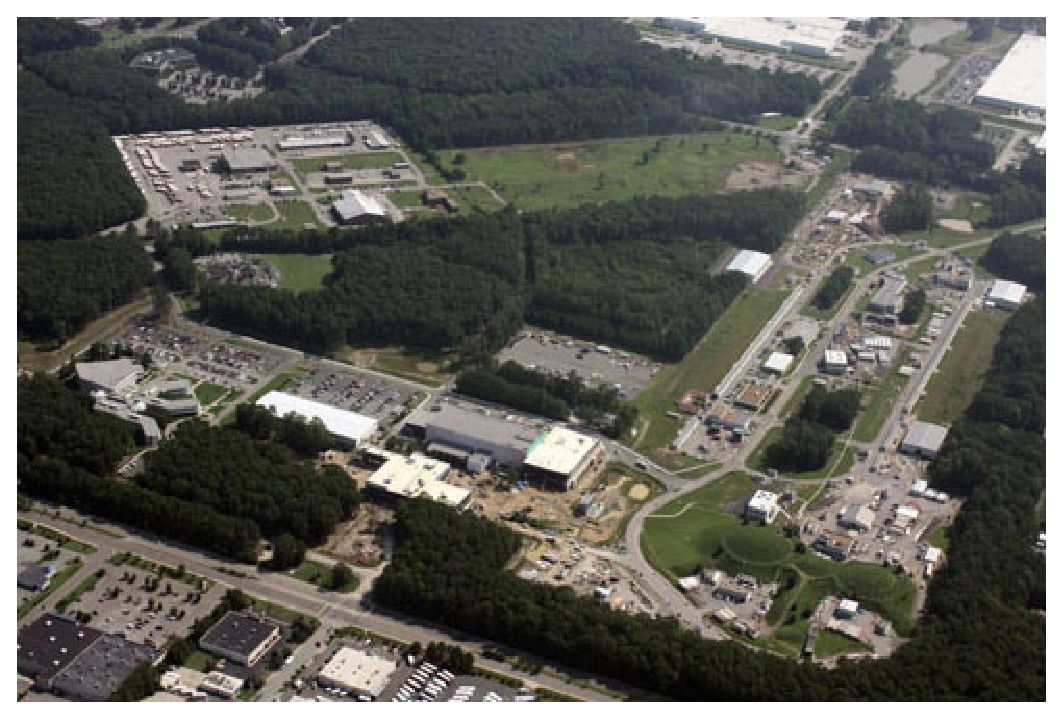
\includegraphics[angle=0, scale=0.85]{./chap1-intro/fig/Visit-JLab3.eps}
%  \end{center}
%  \caption[Aerial view of Jefferson Laboratory, Newport News, Virginia.]{
%    \footnotesize Aerial view of JLab
%  }
%  \label{fig:AerJLab}
%\end{figure}
%
%
%
%Use the label name to refer to  Figure  ~\ref{fig:AerJLab}.
%
%\subsubsection{Sub sub section a}
%
%This is a subsubsection
%
%\subsubsection {Sub sub section b}
%
%Another subsubsection......



\chapter{\bf{The EMC Effect}}             % Chapter  1
%\setcounter{figure}{0}
%\setcounter{table}{0}
%\setcounter{equation}{0}
\section{Yield Calculation}

The MARATHON experiment measured cross section ratios. This method allows us to cancel many systematics that would otherwise plague a full cross section analysis. By taking data for each target at the same kinematics, acceptance effects are identical. This data taking technique means that with reasonable acceptance cuts, a ratio of target yields is wholly equivalent to the ratio of cross sections.

To calculate the yield we use a simple equation:

\begin{equation}
	\text{Yield} = \frac{\text{Counts}}{\text{Scattering Centers} \cdot \text{Livetime}} \cdot \text{Corrections}
\end{equation}

The yield is binned in Bjorken $x$. This chapter will explain the cuts and corrections that go into this calculation.

\section{Calibration}
\subsection{Raster Calibration}
The raster is calibrated by defining a line that maps the raster current to positions at each BPM and the target. To do this, the slope and intercept of this line had to be determined. The slope corresponds to the conversion of raster current to position displacement. The intercept is then determined from the central position that the beam is displaced from. This section will be a general presentation of the techniques used to calibrate the raster. For a more in-depth discussion of how the raster was calibrated, see Appendix \ref{raster_appendix}.

For the horizontal raster, this was done by optimizing the reconstructed z-vertex on the target. When properly calibrated, there should be no correlation between the horizontal raster and the z-vertex. Linear interpolation between two ``bad'' calibrations is a simple way to determine the correct calibration slope.

The veritcal raster could be calibrated in a similar way by minimizing the correlation between the vertical raster and a known momentum phenomena (i.e. a $W^2$ peak). Unfortunately, such a feature does not exist within the kinematics of MARATHON data. The vertical calibration was determined using the carbon hole target. The hole is known to be $2mm$ diameter. By using the raster data, the hole can be fit in order to determine the vertical calibration slope.

The intercepts are determined by looking at the mean BPM position readings and projecting these to the target. This position will correspond to the mean value of the rasters as well. Using the beam position, raster current, and calibration slope the calibration intercept can easily be determined.


\section{Analysis}
\section{Corrections}

When analyzing the data, there are several corrections that need to be made. These are due to various physical or systematic effects that took place during the experiment. These effects have been studied in order to determine a ``correction factor'' that can be applied to the data.

\subsection{Target Boiling}
\label{sec:boiling}

When the beam is incident on the target, it deposits heat into the gas. This causes a density fluctuation of the gas referred to as ``target boiling''. The target does not actually boil, however that is the standard nomenclature for a density fluctuation in a gas target. When the density of the target changes, it changes the effective target thickness as seen by the beam. When the target thickness changes, there is a changed number of scattering centers which will lead to a change in the number of electrons recorded. Specifically, heating will decrease the target density which will decrease the number of scattered electrons.

The density changes are a function of the current on the target. Each run is taken at a single current so that the correction can be applied run by run. The correction is approximately linear for small deviations in current. A study of the effect during beam ramping found that the density settles very quickly. This means that so long as we cut events that occur with the beam off, it is unnecessary to take into account the beam ramping when correcting for this effect.

To determine the correction, a dedicated set of runs was taken with the Left HRS spectrometer at $16.8\degree$ and 3.1 GeV. At this kinematic, several data runs were recorded with varying current between them. Each of these runs were analyzed with the standard data cuts to determine the yield. This allows for the yield to be determined as a function of beam current.

Now that the yields have been determined as a function of beam current, they can be plotted and fit. The data is fit with a quadratic polynomial. This fit is constrained to require no correction (a correction factor of 1) at zero current. This is because the density must be the nominal fill density when there is no beam heating. During analysis the average current is calculated for a run (ignoring beam trips). The average current is then used to calculate the target density correction with the fit function. The correction is then applied on a run-by-run basis by multiplying the number of scattering centers by this correction factor (or equivalently dividing the yield by the correction factor). Figure \ref{fig:boilcor} shows the correction factors for each target.\cite{boiling}

\begin{figure}
	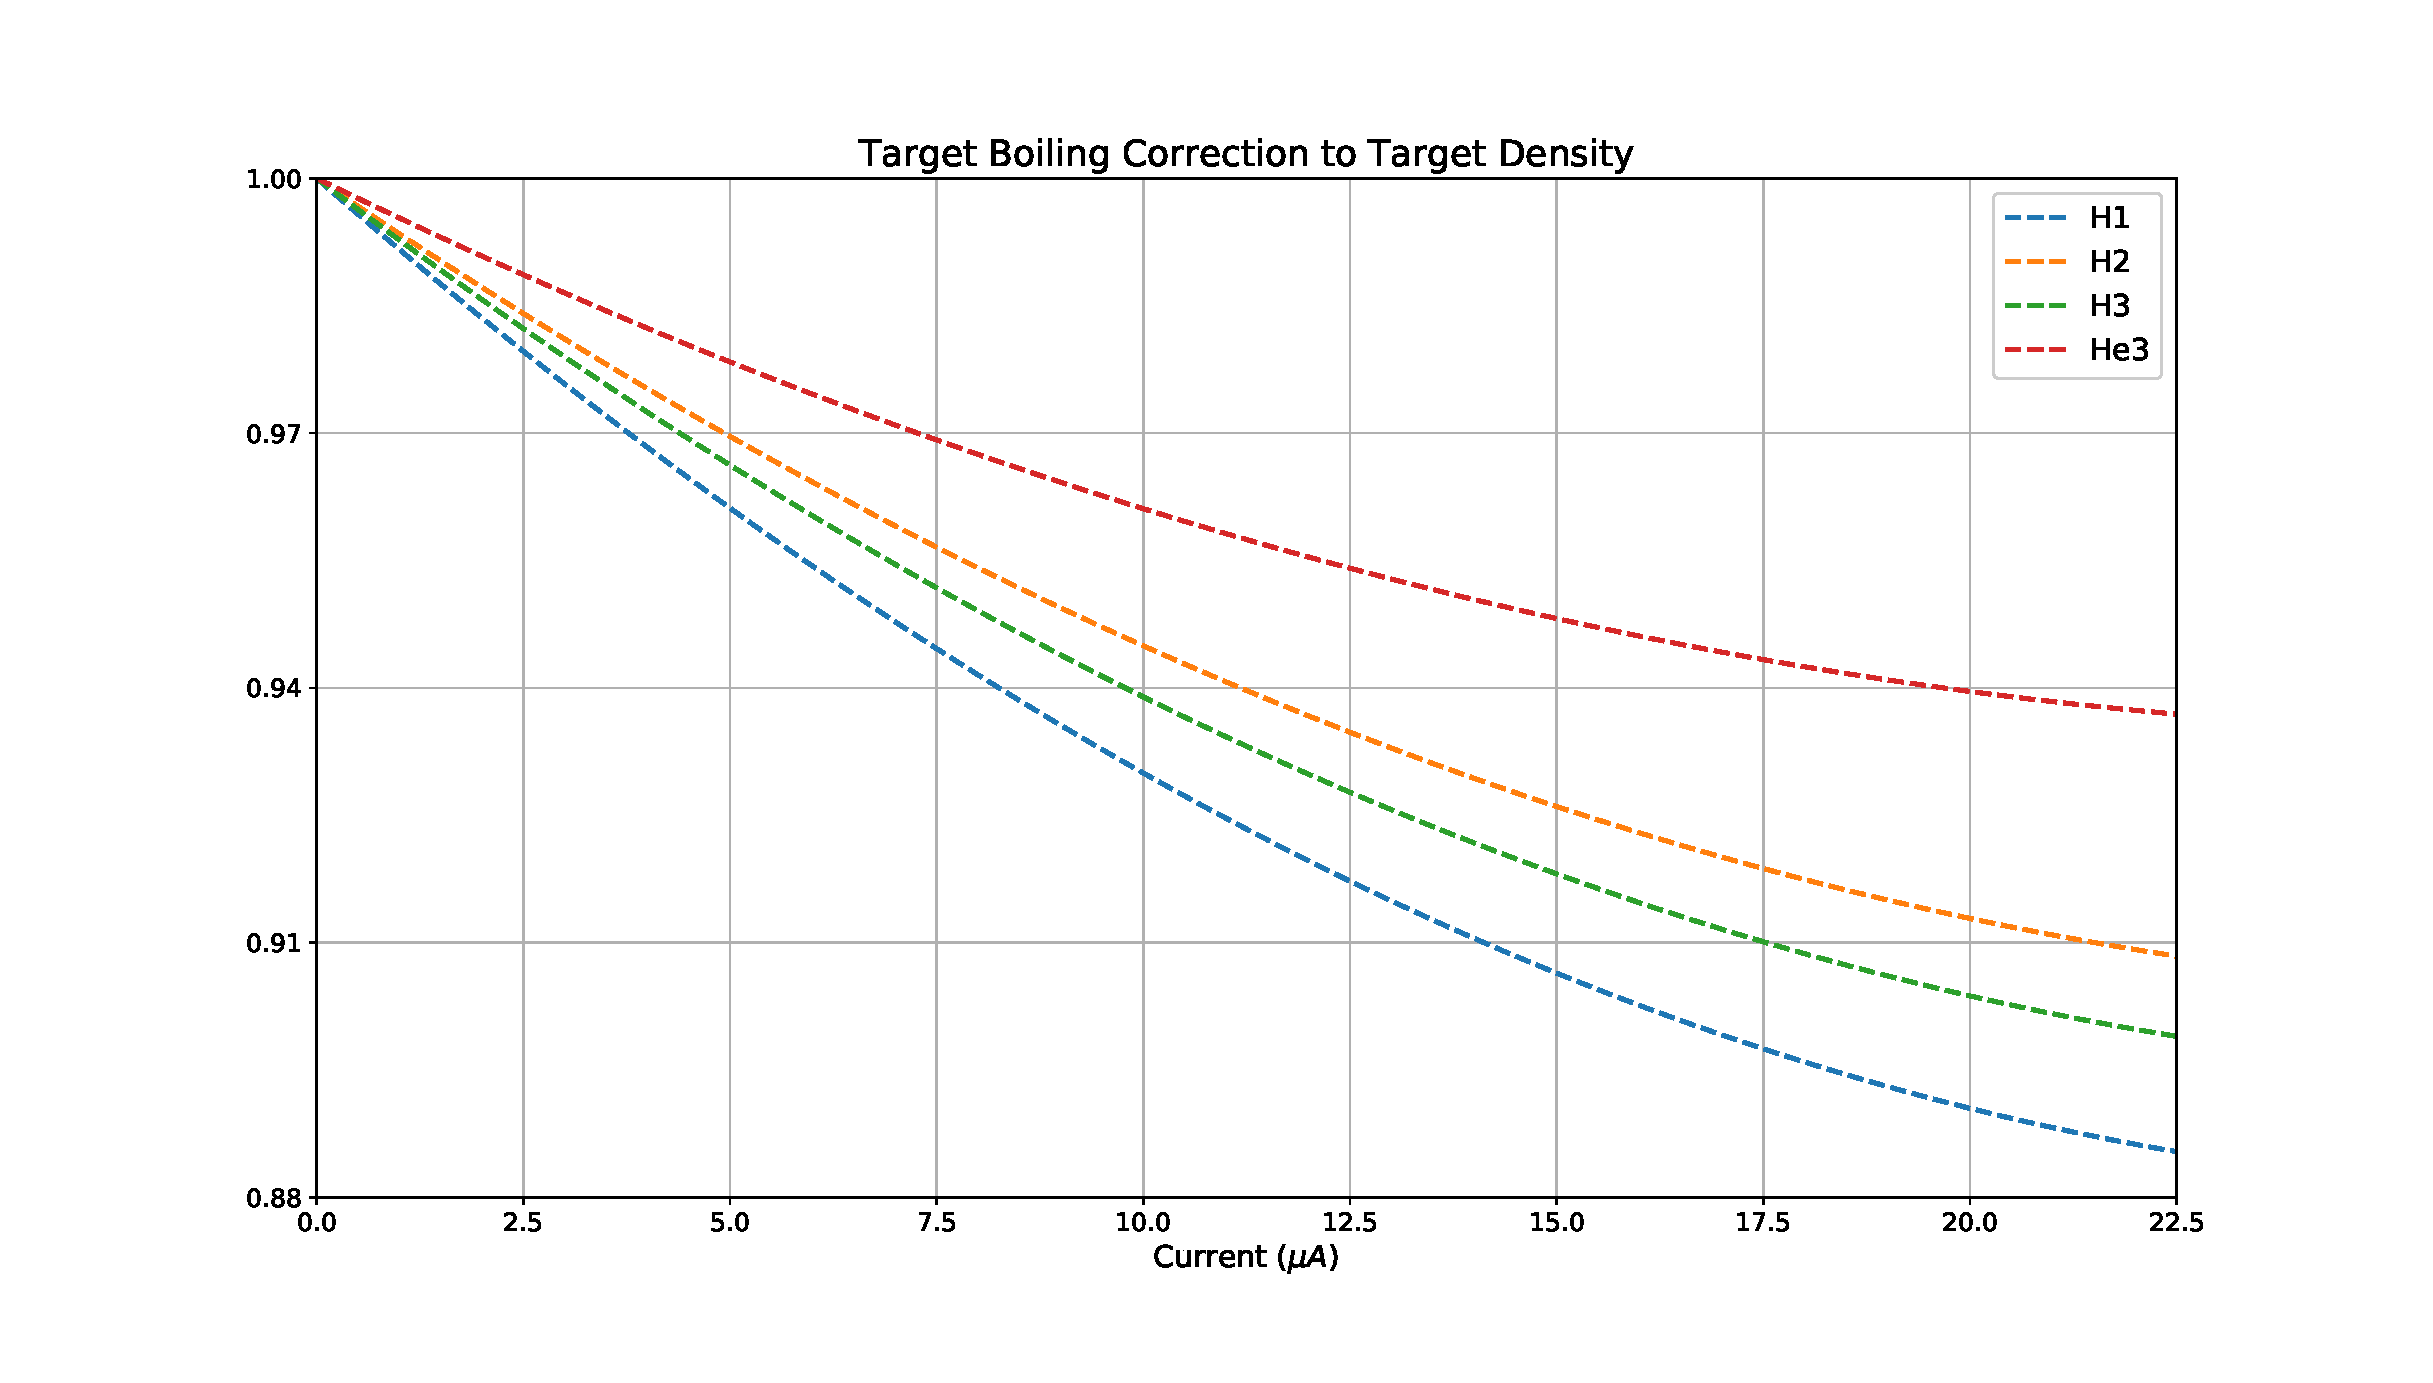
\includegraphics[width=\textwidth]{./analysis/fig/boil_cor.eps}
	\caption{Beam heating effects are manifested as a multiplicative correction to the target density}
	\label{fig:boilcor}
\end{figure}

%\begin{figure}
%	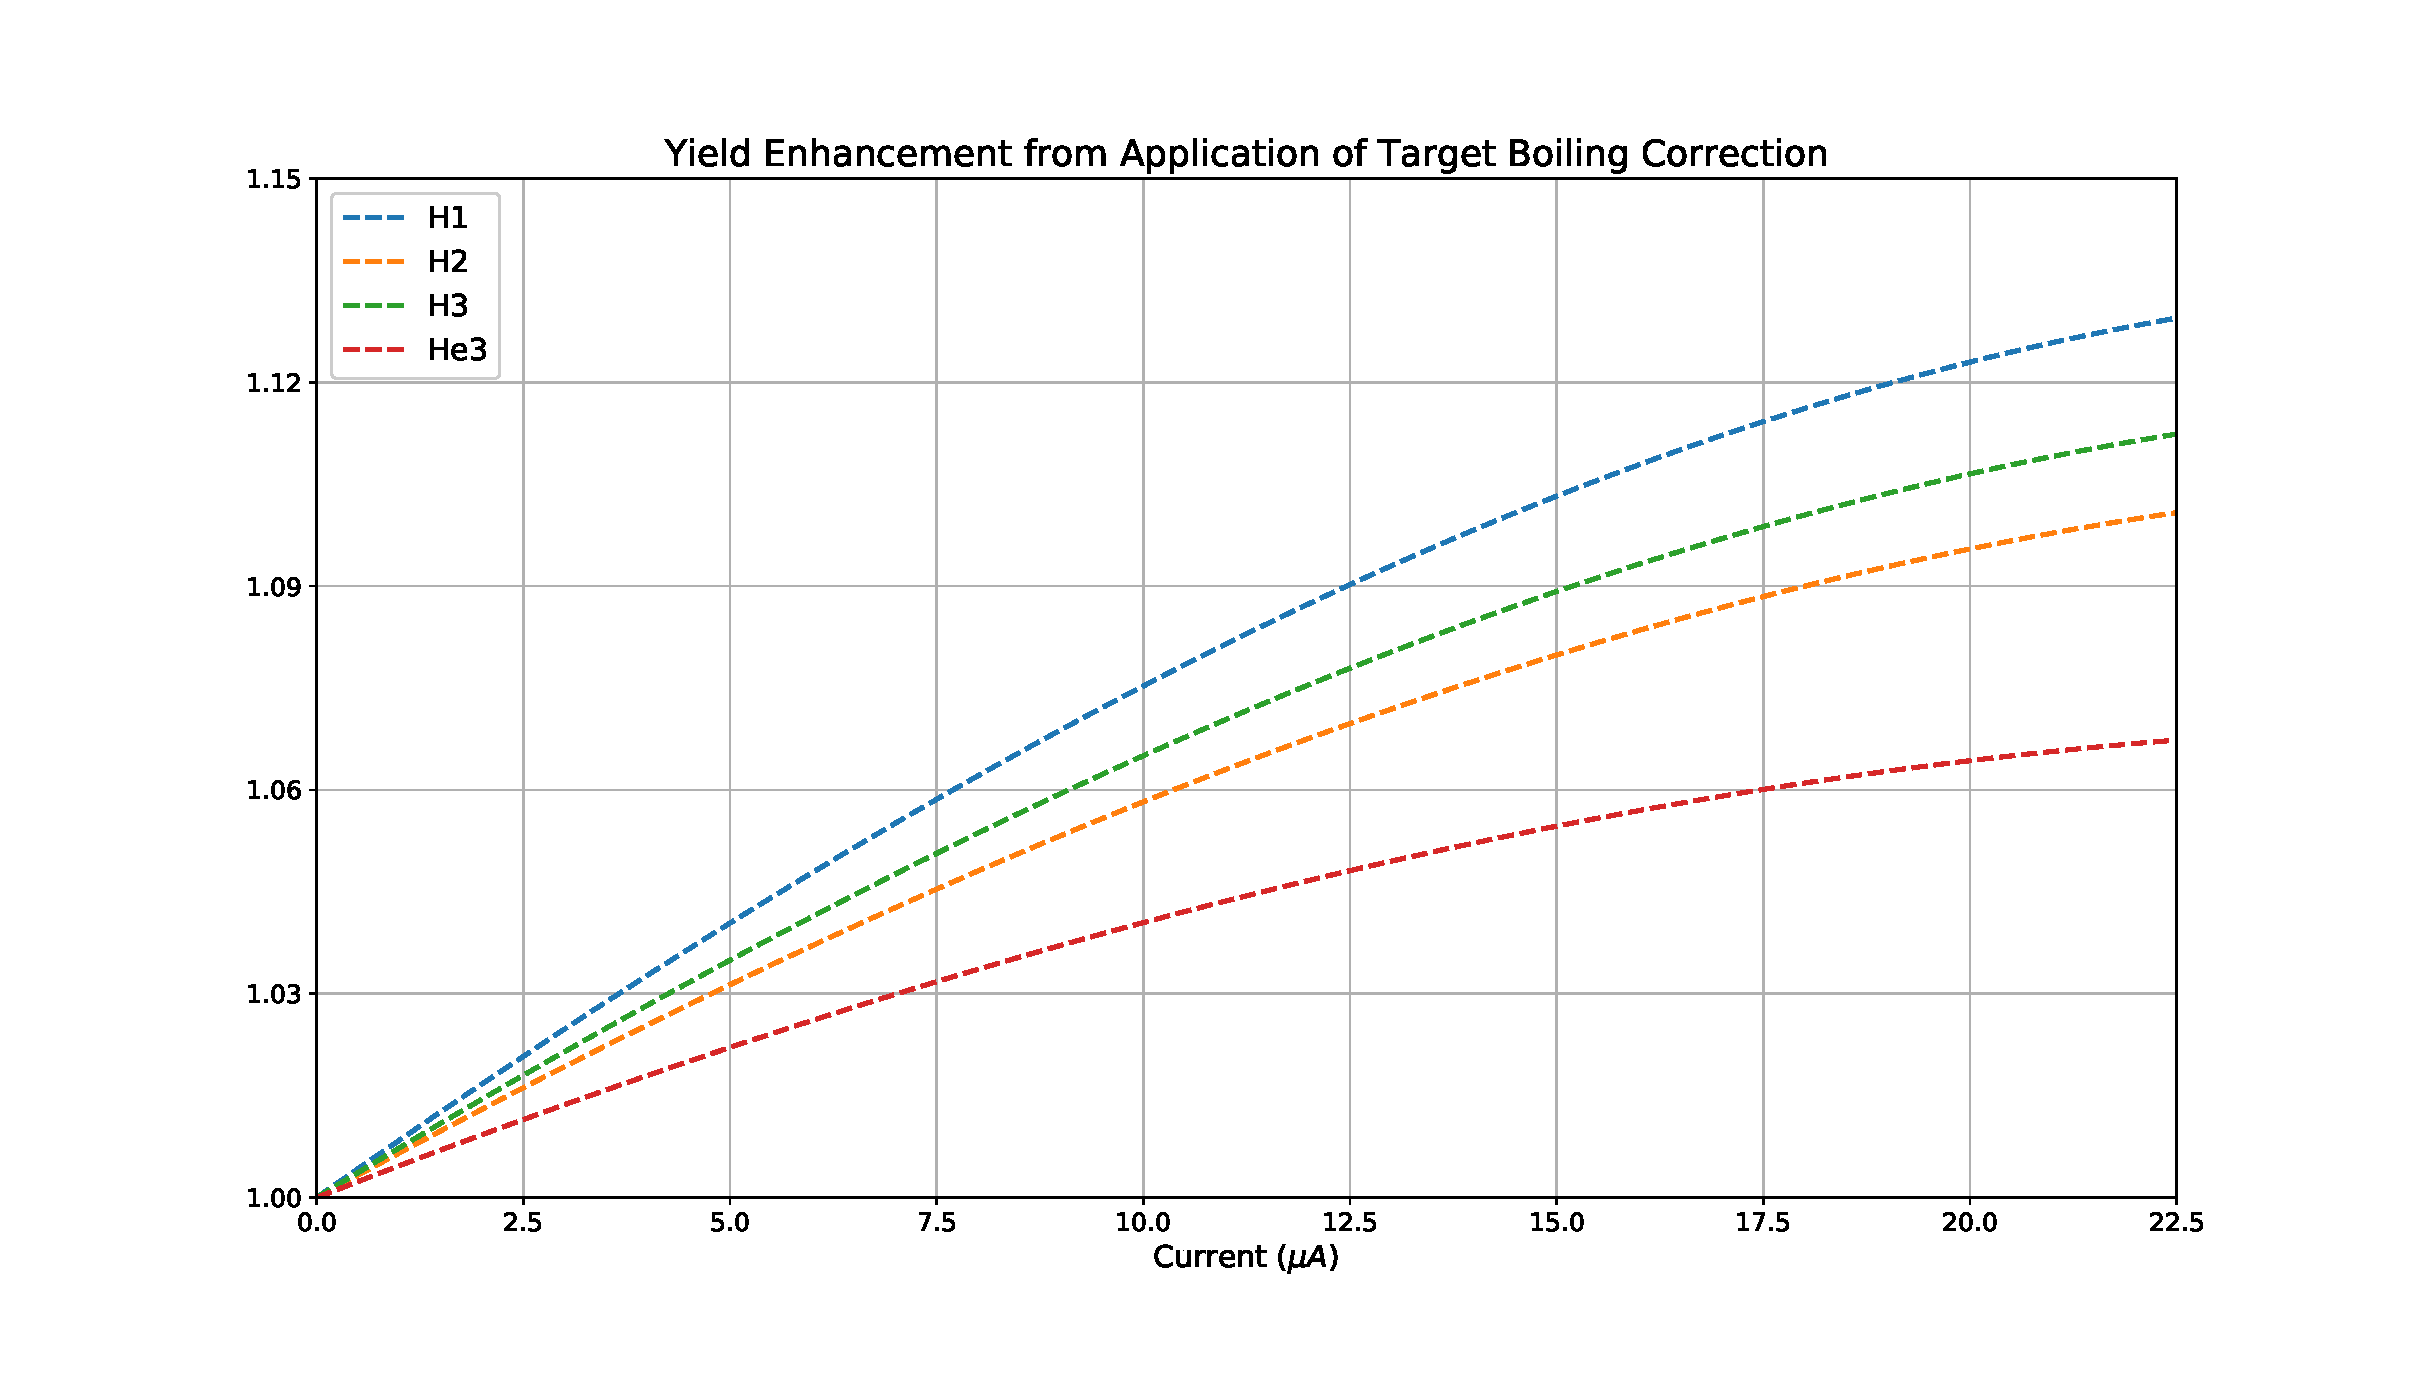
\includegraphics[width=\textwidth]{./analysis/fig/boil_yield_cor.eps}
%	\caption{Target density corrections cause a multiplicative enhancement to the yield}
%	\label{fig:boilyieldcor}
%\end{figure}

\subsection{Target Endcap Contamination}
\label{sec:ecc}

The gas targets used in this experiment are housed in aluminum cells as described in Section \ref{sec:gas_cell}. The thickness of the aluminum greatly exceeds the thickness of the gas and will contribute background that can survive the cuts placed on the data. By quantifying this contribution, the events that originate from the cell endcaps can be subtracted from the final results.

To determine this contribution, the empty cell is used. The empty cell, being an exact replica of the gas target cells with a vacuum inside, allows us to approximately isolate the contribution of the cell walls to the data. The empty cell and the target being studied are compared by calculating the yields on a kinematic-by-kinematic basis and normalizing them by charge and endcap thickness.

The normalization to the endcaps for each target must be done in two parts. This is because each endcap is not the same thickness. When calculating the yield for a target, it is assumed that any contamination upstream (downstream) of the center of the target must originate from the upstream (downstream) endcap. The two halves are then combined to arrive at the endcap thickness normalized yield. This yield calculation only has livetime corrections applied. All cuts are applied except for target length, which is adjusted to only include events upstream (downstream) of the center of the target.

The data for the target being studied and the normalized empty target are then binned in Bjorken $x$. Dividing the empty cell data by the gas target data then gives an approximation of the fractional contribution of the cell walls to the electron data. As this correction is applied to the final results, the contamination corrections for the targets are divided by each other to create the correction to the target ratios. These results are then fit with the functional form $1\pm e^{Ax+B}$. The choice of adding or subtracting the exponential is done by determining if the correction is greater or smaller than 1. The fit function and the covariance matrix of the fit are used to apply the correction to the final results as well as determine the uncertainty contribution of this correction.

\subsection{Charge Symmetric Background Subtraction}

As an inclusive scattering experiment, we are particularly susceptible to background from charge symmetric processes from the target. That is events which involved the production of both an electron and a positron, rather than the electron simply scattering. To study this, the polarity of the LHRS was reversed so that positively charge particles are directed into the detectors rather than negatively charged particles. With this setting, a number of runs were taken in kinematics 0 through 5. These runs were taken with all targets, just as the electron data was taken. This allows for a measurement of the positron yield which corresponds to a measure of the charge symmetric background.

This measurement allows us to determine the proportion of electrons that originated from pair production. Applying the same cuts and as the electron data allows us to determine the charge normalized positron yield. Unlike in the electron analysis, it was noted that there was significant pion contamination in the positron data. This pion contamination had to be subtracted in order to get an accurate calculation of the positron yield. This is achieved by fitting the main pion peak and the subtracting the tail of the fit which survives the cuts applied from the positron data.

The charge normalized positron yields over these kinematics are then combined (using the same methods as the electron yield) and binned in Bjorken $x$. This was then divided by the charge normalized electron yield. This is a fractional measure of the charge normalized background contamination. The ratio is then fit with an exponential of the form $e^{Ax + B}$, where $A$ and $B$ are the fit parameters. These fits are shown in in Figure \ref{fig:positrons}.

This correction is applied to the final yield ratio results. Both the numerator and denominator must have the charge symmetric background subtracted. Each target yield in the ratio is scaled by $1 - \left(\textrm{Charge Symmetric Background Fit}\right)$. For each bin, the fit is calculated at the bin center.

\begin{figure}
	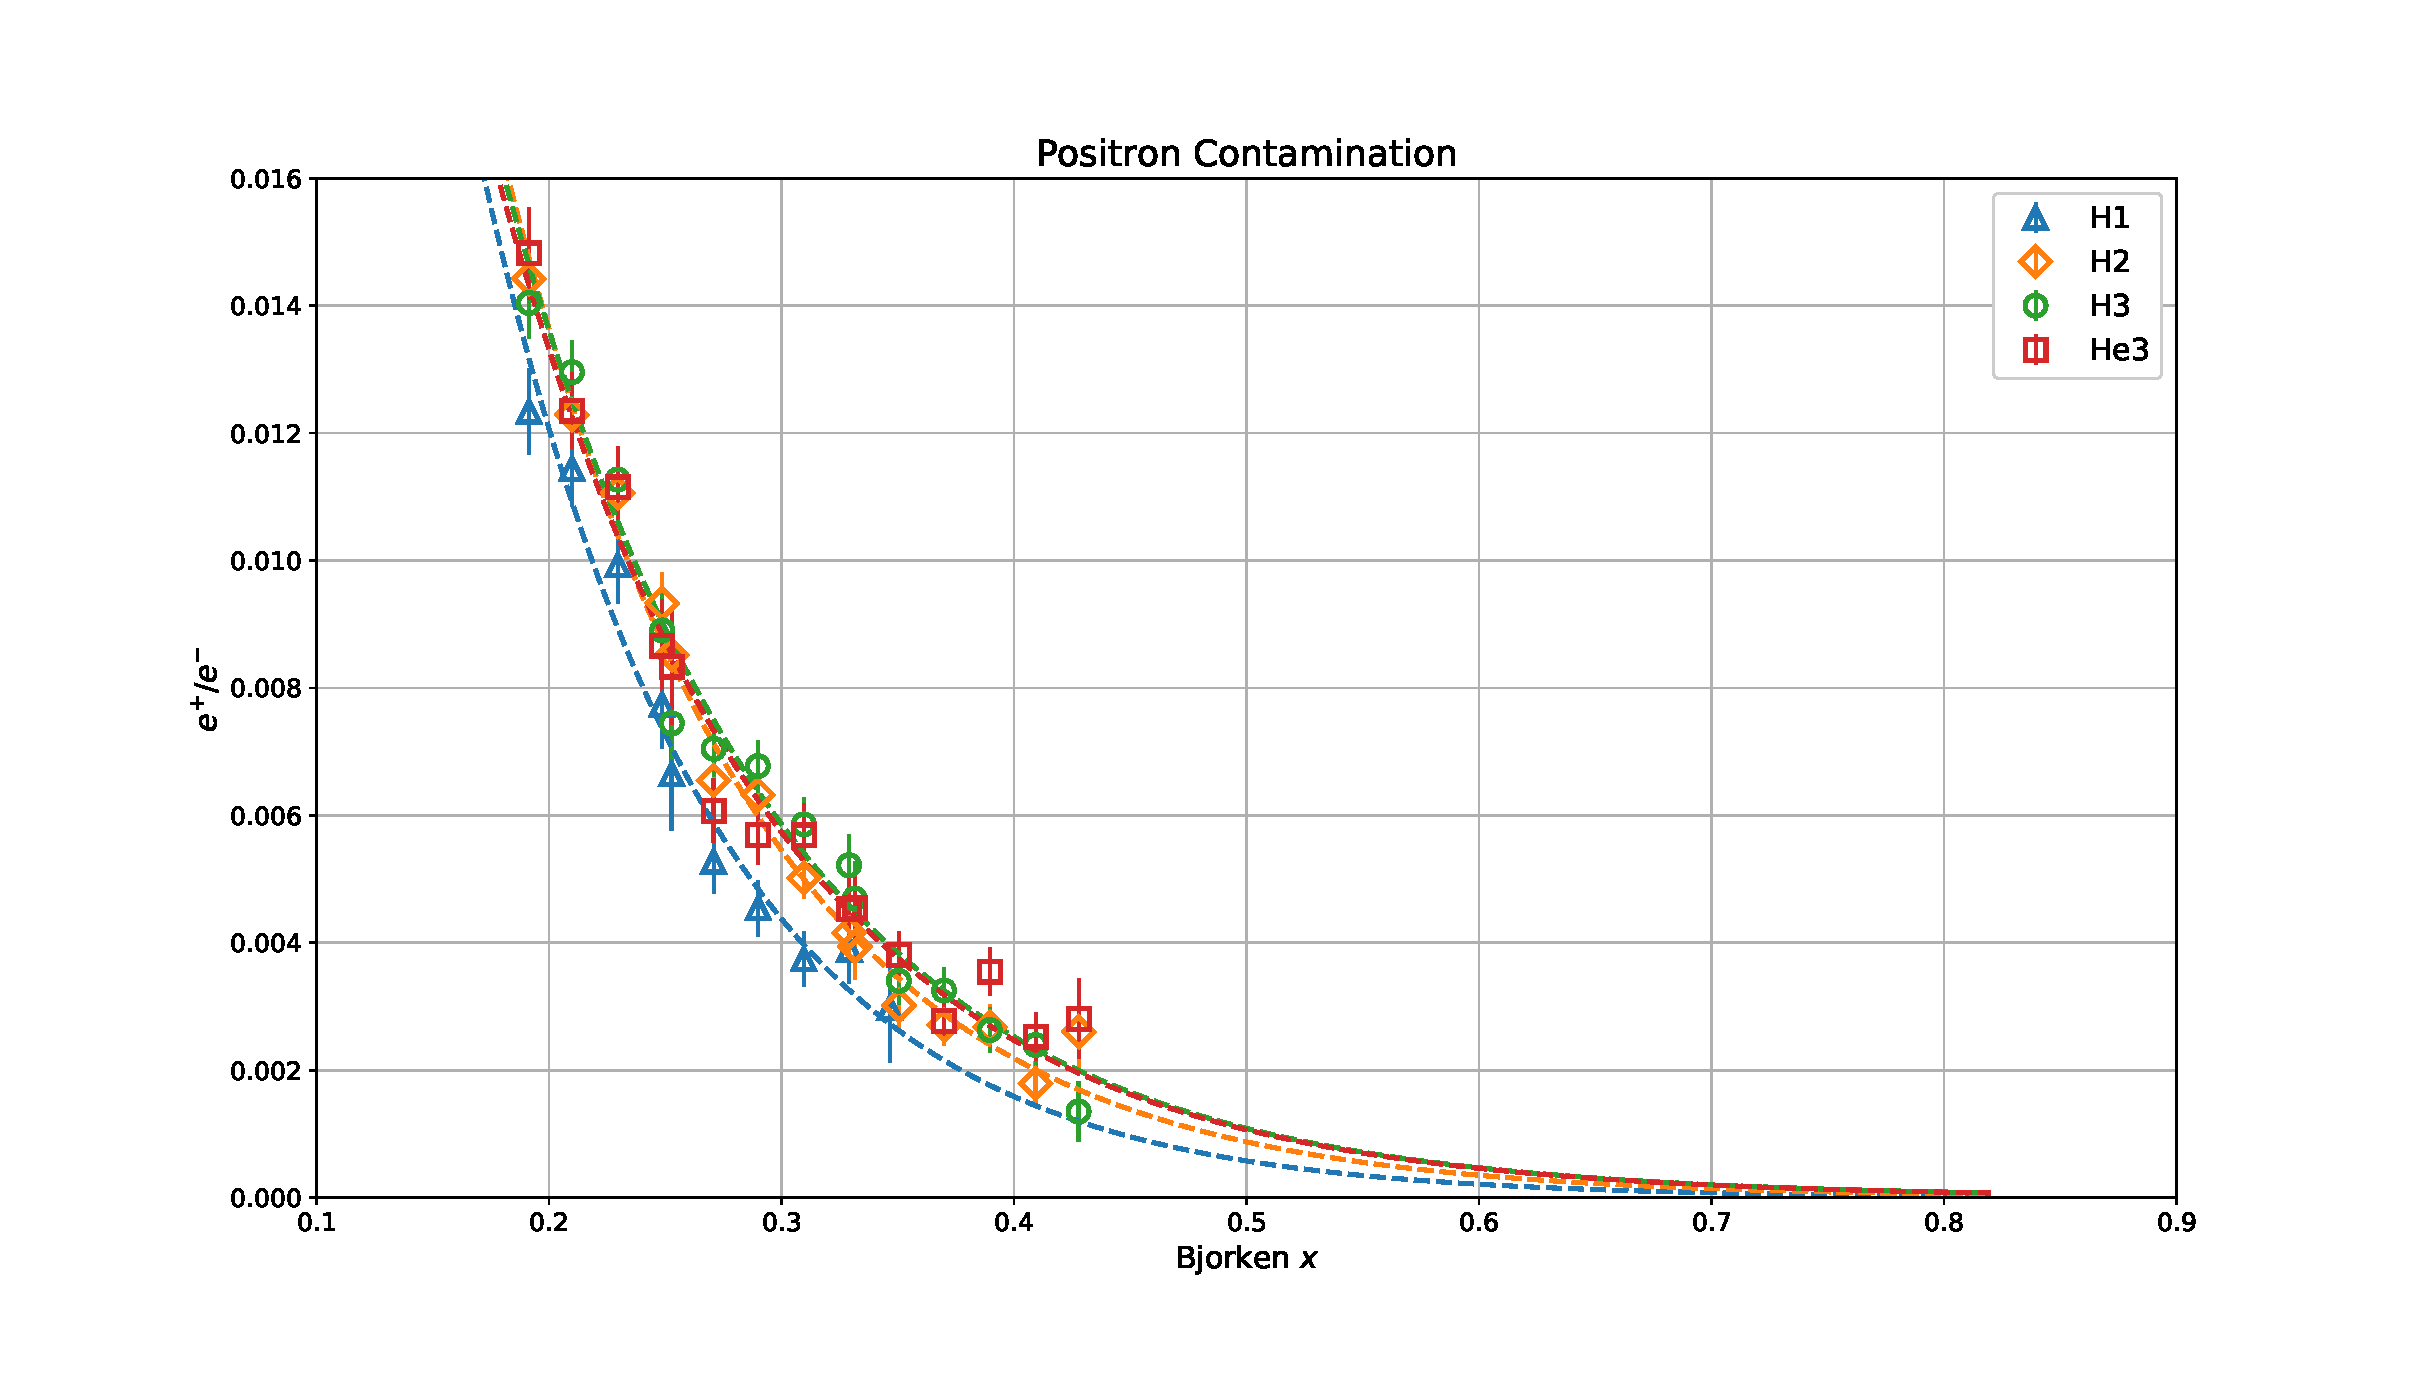
\includegraphics[width=\textwidth]{./analysis/fig/positrons.eps}
	\caption{Charge symmetric background correction}
	\label{fig:positrons}
\end{figure}

\subsection{Computer Deadtime Correction}

Our DAQ unable to continuously record data. While we can probabilistically determine the mean time spacing between events, in the real world events can deviate greatly from these means. Sometimes events will occur that are too close in time for our DAQ to record as the computer has not completed recording the previous event. Deadtime is a function of event rate; when events happen more rapidly, there is a higher chance that events will occur too closely in time to be recorded.

When deadtime is low and the number of recorded events is high, it is a reasonable assumption that the events recorded will accurately reflect the distribution of events in the ``zero-deadtime limit''. In this case correcting for the deadtime is simply done by scaling the number of events by the ``livetime'' of the experiment.

The computer livetime was measured using the Trigger Supervisor and scalers in each HRS. The trigger signals generated from detector signals are copied and sent to both the Trigger Supervisor and a scaler unit. The Trigger Supervisor is subject to the computer deadtime event loss discussed here. The scaler unit, on the other hand, simply increments a register when a trigger signal is received. The ratio of these the number of events recorded by these two systems gives a measure of the livetime of the measurement. The livetime is defined on a run-by-run basis as:

\begin{equation}
DT = \frac{\Sigma \mathrm{Triggers_{TS}}}{\Sigma \mathrm{Triggers_{Scaler}}}
\end{equation}

In an ideal world, the deadtime will be identical for all runs within a kinematic. However, the deadtime is measured on a run-by-run basis and is applied as such in order to account for any deviations from this assumption. The average deadtime for each target in each kinematic is plotted in Figure \ref{fig:deadtime}.

\begin{figure}
	\includegraphics[width=\textwidth]{./analysis/fig/deadtime.eps}
	\caption{Deadtime per kinematic}
	\label{fig:deadtime}
\end{figure}

\subsection{Radiative Corrections}

The Deep Inelastic Cross Sections being studied are the Born approximation of a single-photon exchange. The measurement however, contains contributions from higher order processes that will increase the measured cross section. Using a model, the contributions can be corrected for and removed from the measurement.

The experiment used a software package called $\texttt{T2\_EXTERNALS}$ that calculates both the Born cross section and the radiated cross section for a given target at a kinematic set $(E,E^{\prime} ,\theta )$.

\subsection{Isoscalar Corrections}

\subsection{Bin Centering Corrections}

The cross-section over the width of a bin is not constant. This means that the measurement does not correspond with the true cross section at the center of the bin. Using a model that matches the shape of our data well, the location of the measurement within the bin can be calculated. This is done by calculating the expectation value of the model within that bin and determining the $x$ value corresponding to this value. The expectation value is given by
\begin{equation}
	\langle f_{\rm measured}\rangle = \frac{1}{\Delta x}\int_{x_{\rm low}}^{x_{\rm high}} f\left( x \right) dx,
\end{equation}
where $f$ is a function representing the chosen model. In practice, the $x$ value does not need to be calculated if the data will be reported at the bin center. Rather, the correction is simply the ratio of the model at the bin center. This is written as
\begin{equation}
	\sigma_{\textrm{Bin Centered}} = \frac{f\left(x_{\textrm{Bin Center}}\right)}{\langle f_{\rm measured}\rangle} \sigma_{\rm measured}.
\end{equation}

This correction must be applied to both targets in the ratios. That is, the ratio must be multiplied by the correction to the numerator and divided by the correction to the denominator.\cite{wtsydp}

\subsection{Coulomb Corrections}

Corrections must be made for the effect of the charge of the target on the scattered electron. This interaction causes the $Q^2$ of the event to shift to an effective $Q^2$ value, $Q^2_{\rm eff}$. This conversion is done with the equation
\begin{equation}
	Q^2_{\rm eff} = Q^2 \left(1 + \frac{3Z\alpha\hbar c}{2RE}\right)^{2}.
\end{equation}
In this equation $R$ is the hard-sphere equivalent radius of the nucleus which is defined as $R=\left[\left(\nicefrac{5}{3}\right) \langle r^{2}\rangle\right]^{\nicefrac{1}{2}}$ where $\langle r^2\rangle$ is the root-mean-squared radius of the nucleus.\cite{coulomb}

Using $x=\frac{Q^2}{2M\nu}$, it is clear that a shift in $Q^2$ will result in a proportional shift in $x$. Using a model cross-section, the cross section is calculated at both the nominal $x$ and at $x_{\rm eff}$. As the results have been bin centered, this calculation uses a nominal $x$ at the center of the bin. This will lead to the correction
\begin{equation}
	\sigma_{\textrm{Coulomb Corrected}} = \sigma_{\rm data} \frac{\sigma_{\rm model}\left(x_{\rm eff}\right)}{\sigma_{\rm model}\left(x\right)}.
\end{equation}

This correction must be applied to both targets in the ratios that are calculated.
\subsection{Particle Identification}


%\chapter{\bf{The Experiment}}    % Chapter  2
%%\setcounter{figure}{0}
%%\setcounter{table}{0}
%%\setcounter{equation}{0}
%\section{The Measurement}
\subsection{What are we measuring}
\subsection{How are we measuring it}
\subsection{Run Plan}

\section{The Apparatus}
\subsection{Hall A HRS Spectrometers}
\subsection{CEBAF Accelerator}

% \chapter{\bf{Chapter 2 Title}    % Chapter  2
%Introductory paragraph of Chapter 2.......
%
%\section{First section Title}
%
%First section text......
%
%
%
%\subsection{First Subsection Title}
%
%
%The cross section for elastic electron scattering from the spin one-half
%$^3$H  nucleus is given, in the one-photon exchange approximation, by:
%\beqn
%{  {d\sigma} \over {d\Omega} } (E,\Theta)  =
%{  {(Z\alpha)^2 E^\prime} \over {4 E^3  \sin^4 \left( {\Theta \over 2} \right)}  }
%\left[ A(Q^2) \cos^2 \left( {\Theta \over 2} \right) +
%B(Q^2) \sin^2 \left( {\Theta \over 2} \right) \right],
%\label{morefequ}
%\eeqn
%where $Z$ is the nuclear charge, $\alpha$ is the fine-structure constant,
%$E$ and $E'$ are the incident and scattered electron energies,
%$\Theta$ is the electron scattering angle, $Q^2 = 4 E E' \sin^2 (\Theta/2)$ is
%minus the squared four-momentum transfer,
%and $A(Q^2)$ and $B(Q^2)$ are the $^3$H elastic structure functions, given in
%terms of the charge and magnetic form factors as:
%\beqn
%{   A(Q^2) = {   { F^2_C(Q^2) +
%(1+\kappa)^2 \tau F^2_M(Q^2) } \over {1 + \tau} }    },
%\label{more1}
%\eeqn
%\beqn
%{ B(Q^2) =  2 \tau (1+\kappa)^2 F^2_M(Q^2) },
%\label{more2}
%\eeqn
%where
%$\tau=Q^2/4M^2$ with $M$ being the mass of the target nucleus, and
%$\kappa$ is the anomalous magnetic moment of the nucleus.
%
%Here is a reference ~\cite{mara} which needs to be defined in the bibliography.tex file first.
%
%
%Here comes a Figure....
%
% \begin{figure}[!htbp]
%  \begin{center}
%    \includegraphics[angle=90, scale=0.65]{./chap2-exp/fig/tritium_past.eps}
%  \end{center}
%  \caption[Tritium Magnetic Form Factor Past Data]{
%    \footnotesize Tritium Mag. Form Factor past data.
%  }
%  \label{fig:TritiumM}
%\end{figure}
%
%Use the label name to refer to  Figure  ~\ref{fig:TritiumM}.
%
%
%\subsection{Second Subsection  Title}
%
%Subsection text..........
%
%
%
%\subsubsection{First Subsubsection}
%
%This is a subsubsection.
%
%
%
%\subsubsection{Second Subsubsection}
%
%This another  subsubsection.

\setcounter{figure}{0}
\setcounter{table}{0}
\setcounter{equation}{0}
\subsection{Raster}
%Put this in order they appear in beamline?
\section{Beamline Components}

The Hall A Beamline has several measurement devices that allow the experimenter to fully understand the beam that is being delivered to the hall. For positioning, there are the Beam Position Monitors and the Harp. For beamspot sizing, there is the raster. For current and charge measurements, there are the Beam Current Monitors.

\subsection{Beam Position Monitors}

The Beam Position Monitors (BPMs) are a pair of measurement devices that consist of four sensing wires. By calibrating the signal received from each wire, the experimenter can reconstruct the position of the beam as it passed the BPM. Using both BPMs in conjunction allows the experimenter to determine the beam trajectory and where the electrons are incident on the target.

The BPMs are calibrated using a Harp fork. The Harp consists of three wires that are introduced sequentially into the path of the beam using a stepper motor. When the beam is incident on a wire, a charge is induced. By determining when each wire is struck by the beam, the experimenter can very accurately determine the position of the beam. This is an invasive measurement.

\subsection{Raster}
\begin{figure}
	\includegraphics[width=\linewidth]{./chap2-exp/fig/raster_pic.jpg}
	\caption{The Hall A raster consists of four dipole magnets on the beamline}
	\label{fig:raster}
\end{figure}

The raster is a beamline apparatus in Hall A for spreading the beam onto the target, rather than being at a single point. This is done to prevent localized heating of the target. The raster consists of four dipole magnets, two for steering in the x-direction and two for steering in the y-direction.

Each raster magnet is powered by a triangle wave of different frequencies to minimize harmonics. The horizontal rasters are set to 24.5 kHz and the vertical rasters are set to 25 kHz. When running properly, the x-direction magnets will be synced and the y-direction magnets will be synced. This syncing ensures that the magnets are always working together to create the desired beam spread.

\begin{figure}
	\includegraphics[width=\linewidth]{./chap2-exp/fig/raster_sync.png}
	\caption{The X and Y raster pairs are each synced to produce the maximum kick. The X and Y directions are uncorrelated so that the beam travels uniformly over the target.}
	\label{fig:raster}
\end{figure}

\subsection{Beam Current Monitors}


%\chapter{\bf{Analysis}}    % Chapter  3
%%\setcounter{figure}{0}
%%\setcounter{table}{0}
%%\setcounter{equation}{0}
%\section{Yield Calculation}

The MARATHON experiment measured cross section ratios. This method allows us to cancel many systematics that would otherwise plague a full cross section analysis. By taking data for each target at the same kinematics, acceptance effects are identical. This data taking technique means that with reasonable acceptance cuts, a ratio of target yields is wholly equivalent to the ratio of cross sections.

To calculate the yield we use a simple equation:

\begin{equation}
	\text{Yield} = \frac{\text{Counts}}{\text{Scattering Centers} \cdot \text{Livetime}} \cdot \text{Corrections}
\end{equation}

The yield is binned in Bjorken $x$. This chapter will explain the cuts and corrections that go into this calculation.

\section{Calibration}
\subsection{Raster Calibration}
The raster is calibrated by defining a line that maps the raster current to positions at each BPM and the target. To do this, the slope and intercept of this line had to be determined. The slope corresponds to the conversion of raster current to position displacement. The intercept is then determined from the central position that the beam is displaced from. This section will be a general presentation of the techniques used to calibrate the raster. For a more in-depth discussion of how the raster was calibrated, see Appendix \ref{raster_appendix}.

For the horizontal raster, this was done by optimizing the reconstructed z-vertex on the target. When properly calibrated, there should be no correlation between the horizontal raster and the z-vertex. Linear interpolation between two ``bad'' calibrations is a simple way to determine the correct calibration slope.

The veritcal raster could be calibrated in a similar way by minimizing the correlation between the vertical raster and a known momentum phenomena (i.e. a $W^2$ peak). Unfortunately, such a feature does not exist within the kinematics of MARATHON data. The vertical calibration was determined using the carbon hole target. The hole is known to be $2mm$ diameter. By using the raster data, the hole can be fit in order to determine the vertical calibration slope.

The intercepts are determined by looking at the mean BPM position readings and projecting these to the target. This position will correspond to the mean value of the rasters as well. Using the beam position, raster current, and calibration slope the calibration intercept can easily be determined.


\section{Analysis}
\section{Corrections}

When analyzing the data, there are several corrections that need to be made. These are due to various physical or systematic effects that took place during the experiment. These effects have been studied in order to determine a ``correction factor'' that can be applied to the data.

\subsection{Target Boiling}
\label{sec:boiling}

When the beam is incident on the target, it deposits heat into the gas. This causes a density fluctuation of the gas referred to as ``target boiling''. The target does not actually boil, however that is the standard nomenclature for a density fluctuation in a gas target. When the density of the target changes, it changes the effective target thickness as seen by the beam. When the target thickness changes, there is a changed number of scattering centers which will lead to a change in the number of electrons recorded. Specifically, heating will decrease the target density which will decrease the number of scattered electrons.

The density changes are a function of the current on the target. Each run is taken at a single current so that the correction can be applied run by run. The correction is approximately linear for small deviations in current. A study of the effect during beam ramping found that the density settles very quickly. This means that so long as we cut events that occur with the beam off, it is unnecessary to take into account the beam ramping when correcting for this effect.

To determine the correction, a dedicated set of runs was taken with the Left HRS spectrometer at $16.8\degree$ and 3.1 GeV. At this kinematic, several data runs were recorded with varying current between them. Each of these runs were analyzed with the standard data cuts to determine the yield. This allows for the yield to be determined as a function of beam current.

Now that the yields have been determined as a function of beam current, they can be plotted and fit. The data is fit with a quadratic polynomial. This fit is constrained to require no correction (a correction factor of 1) at zero current. This is because the density must be the nominal fill density when there is no beam heating. During analysis the average current is calculated for a run (ignoring beam trips). The average current is then used to calculate the target density correction with the fit function. The correction is then applied on a run-by-run basis by multiplying the number of scattering centers by this correction factor (or equivalently dividing the yield by the correction factor). Figure \ref{fig:boilcor} shows the correction factors for each target.\cite{boiling}

\begin{figure}
	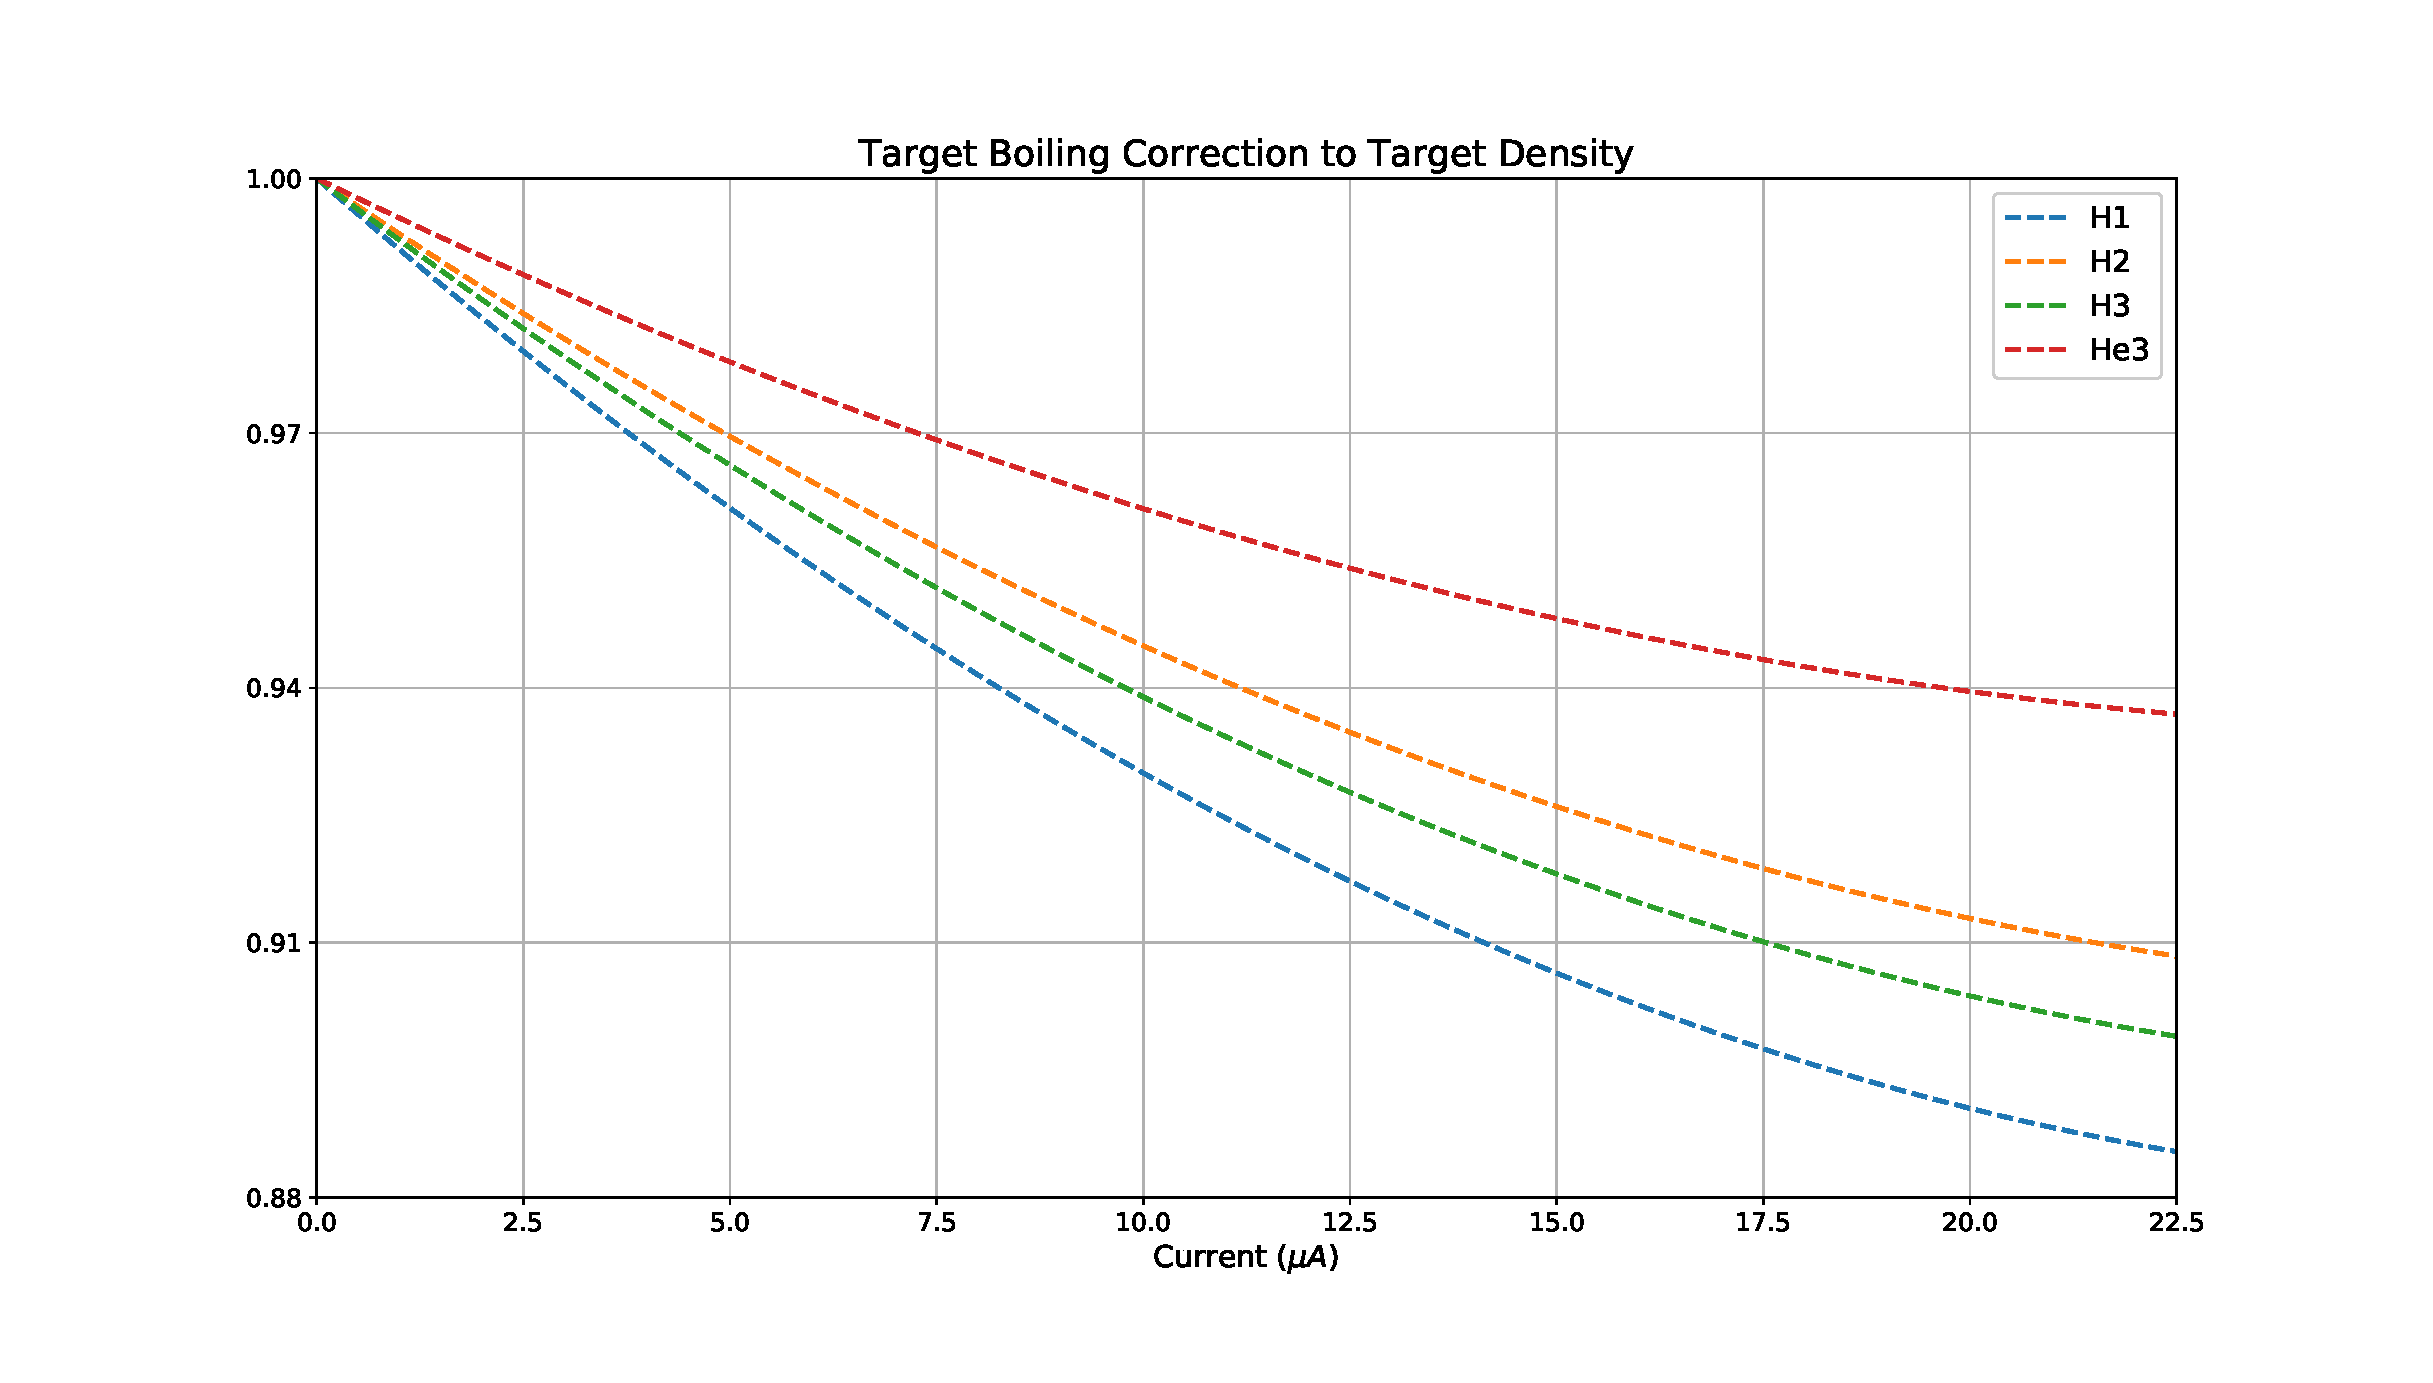
\includegraphics[width=\textwidth]{./analysis/fig/boil_cor.eps}
	\caption{Beam heating effects are manifested as a multiplicative correction to the target density}
	\label{fig:boilcor}
\end{figure}

%\begin{figure}
%	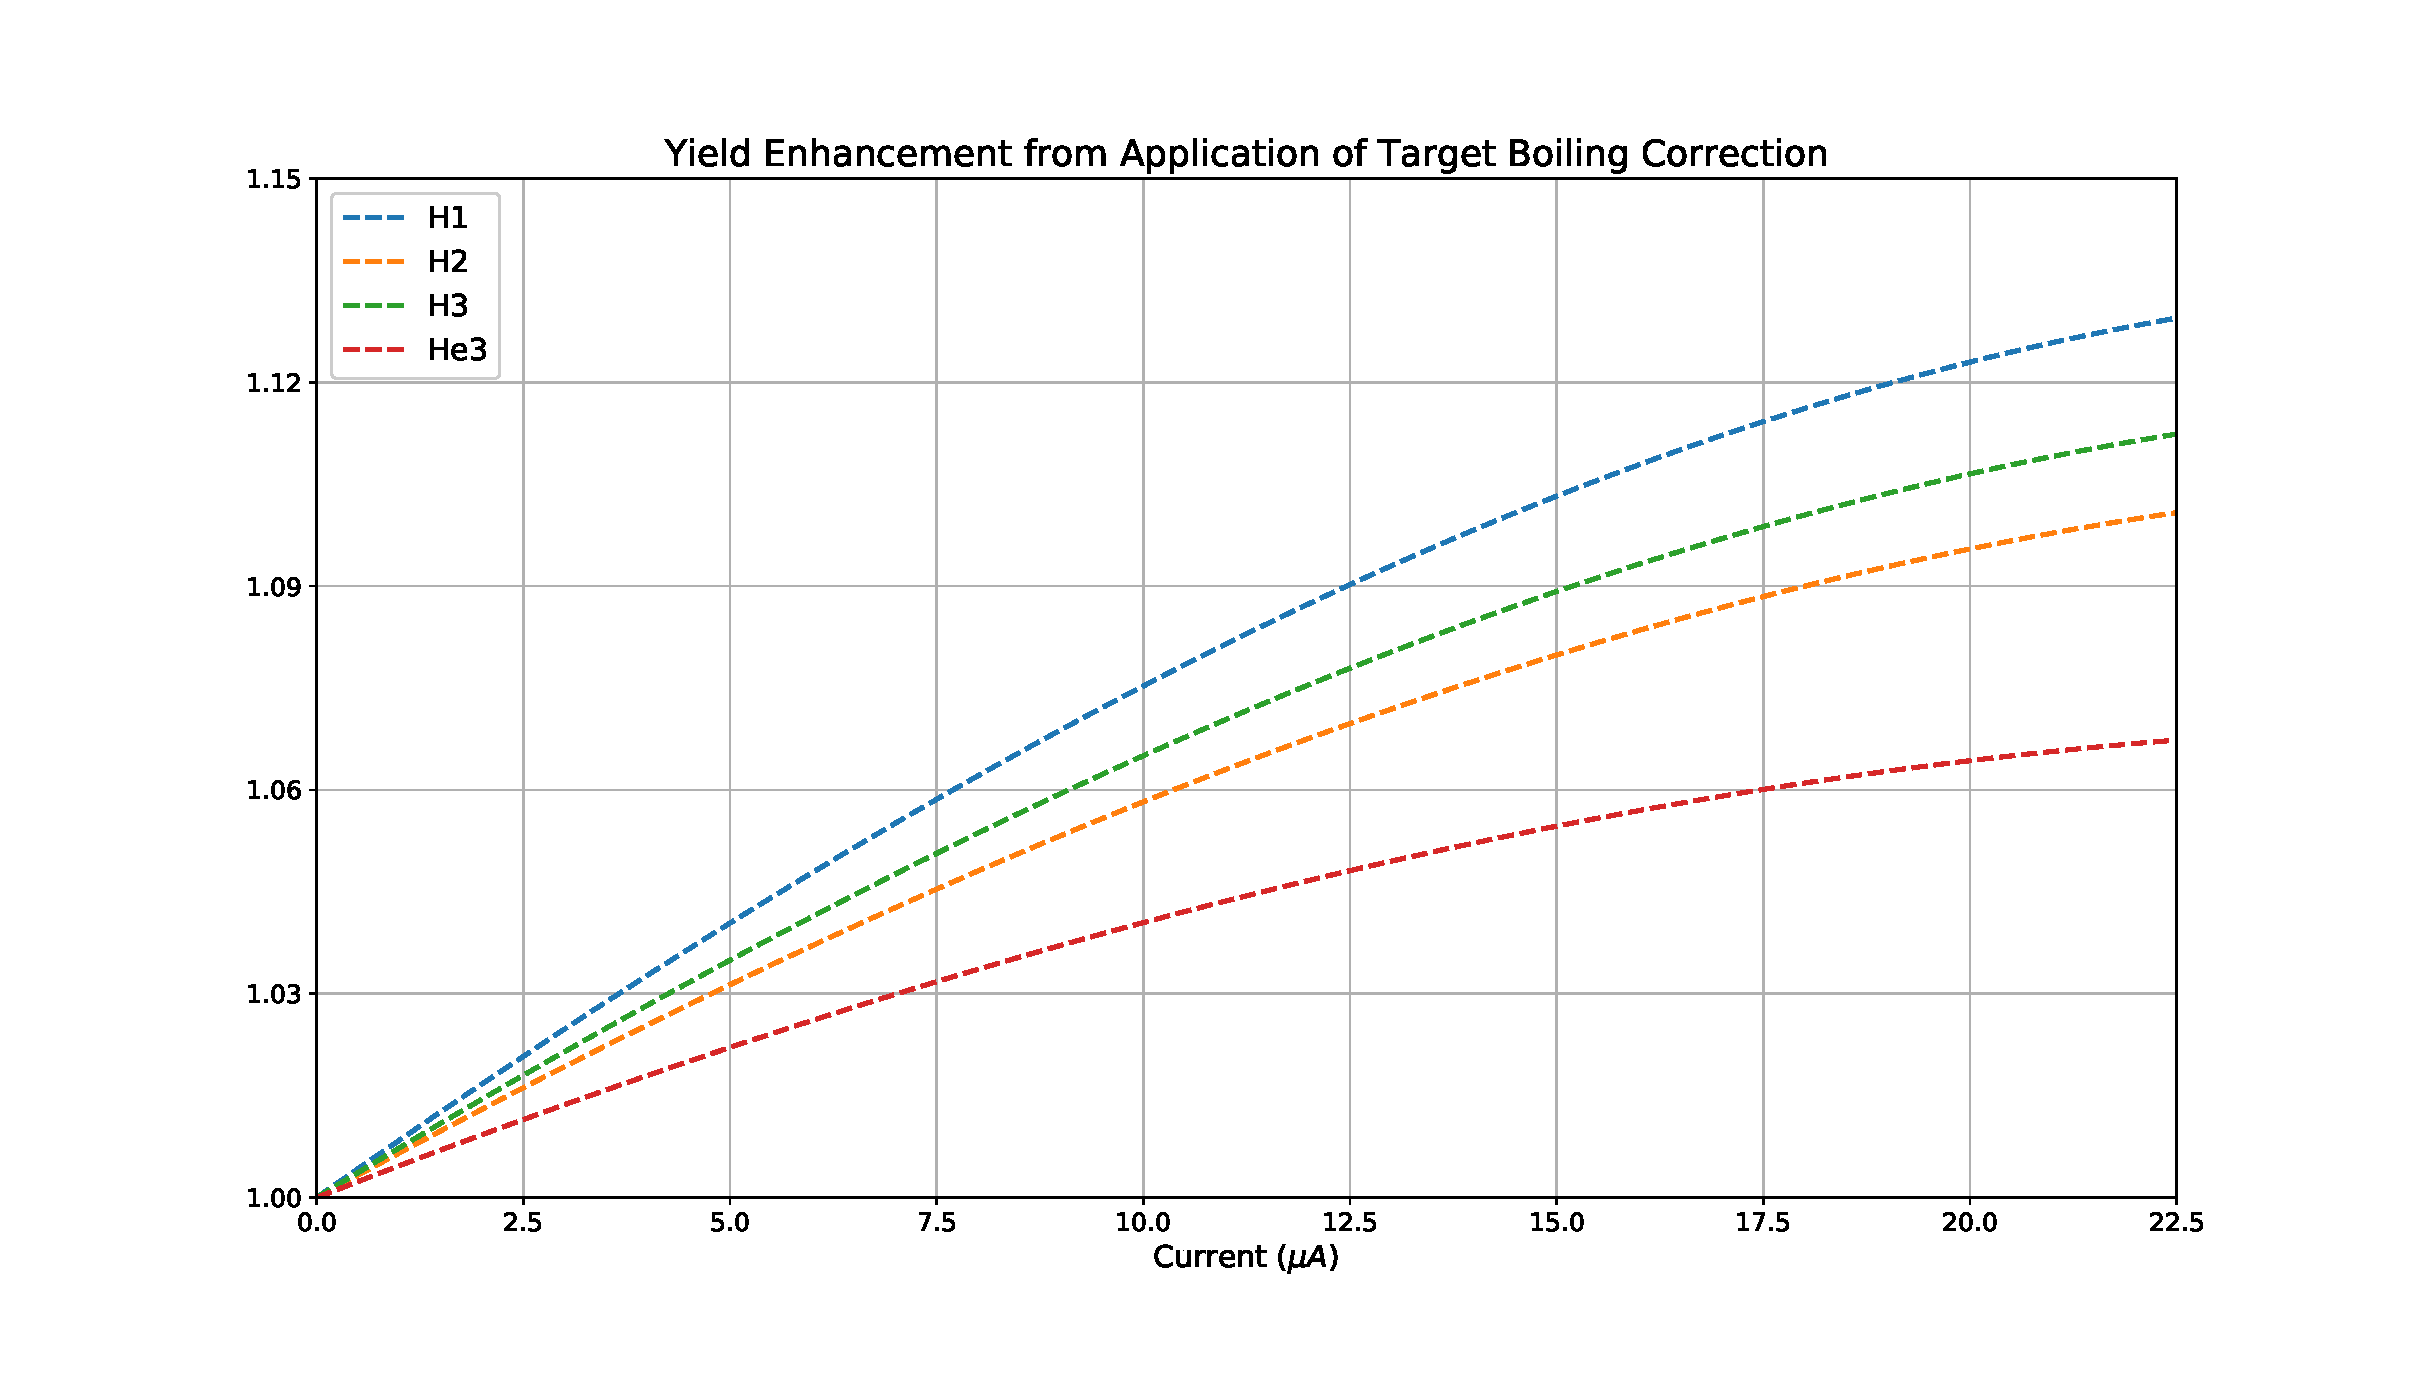
\includegraphics[width=\textwidth]{./analysis/fig/boil_yield_cor.eps}
%	\caption{Target density corrections cause a multiplicative enhancement to the yield}
%	\label{fig:boilyieldcor}
%\end{figure}

\subsection{Target Endcap Contamination}
\label{sec:ecc}

The gas targets used in this experiment are housed in aluminum cells as described in Section \ref{sec:gas_cell}. The thickness of the aluminum greatly exceeds the thickness of the gas and will contribute background that can survive the cuts placed on the data. By quantifying this contribution, the events that originate from the cell endcaps can be subtracted from the final results.

To determine this contribution, the empty cell is used. The empty cell, being an exact replica of the gas target cells with a vacuum inside, allows us to approximately isolate the contribution of the cell walls to the data. The empty cell and the target being studied are compared by calculating the yields on a kinematic-by-kinematic basis and normalizing them by charge and endcap thickness.

The normalization to the endcaps for each target must be done in two parts. This is because each endcap is not the same thickness. When calculating the yield for a target, it is assumed that any contamination upstream (downstream) of the center of the target must originate from the upstream (downstream) endcap. The two halves are then combined to arrive at the endcap thickness normalized yield. This yield calculation only has livetime corrections applied. All cuts are applied except for target length, which is adjusted to only include events upstream (downstream) of the center of the target.

The data for the target being studied and the normalized empty target are then binned in Bjorken $x$. Dividing the empty cell data by the gas target data then gives an approximation of the fractional contribution of the cell walls to the electron data. As this correction is applied to the final results, the contamination corrections for the targets are divided by each other to create the correction to the target ratios. These results are then fit with the functional form $1\pm e^{Ax+B}$. The choice of adding or subtracting the exponential is done by determining if the correction is greater or smaller than 1. The fit function and the covariance matrix of the fit are used to apply the correction to the final results as well as determine the uncertainty contribution of this correction.

\subsection{Charge Symmetric Background Subtraction}

As an inclusive scattering experiment, we are particularly susceptible to background from charge symmetric processes from the target. That is events which involved the production of both an electron and a positron, rather than the electron simply scattering. To study this, the polarity of the LHRS was reversed so that positively charge particles are directed into the detectors rather than negatively charged particles. With this setting, a number of runs were taken in kinematics 0 through 5. These runs were taken with all targets, just as the electron data was taken. This allows for a measurement of the positron yield which corresponds to a measure of the charge symmetric background.

This measurement allows us to determine the proportion of electrons that originated from pair production. Applying the same cuts and as the electron data allows us to determine the charge normalized positron yield. Unlike in the electron analysis, it was noted that there was significant pion contamination in the positron data. This pion contamination had to be subtracted in order to get an accurate calculation of the positron yield. This is achieved by fitting the main pion peak and the subtracting the tail of the fit which survives the cuts applied from the positron data.

The charge normalized positron yields over these kinematics are then combined (using the same methods as the electron yield) and binned in Bjorken $x$. This was then divided by the charge normalized electron yield. This is a fractional measure of the charge normalized background contamination. The ratio is then fit with an exponential of the form $e^{Ax + B}$, where $A$ and $B$ are the fit parameters. These fits are shown in in Figure \ref{fig:positrons}.

This correction is applied to the final yield ratio results. Both the numerator and denominator must have the charge symmetric background subtracted. Each target yield in the ratio is scaled by $1 - \left(\textrm{Charge Symmetric Background Fit}\right)$. For each bin, the fit is calculated at the bin center.

\begin{figure}
	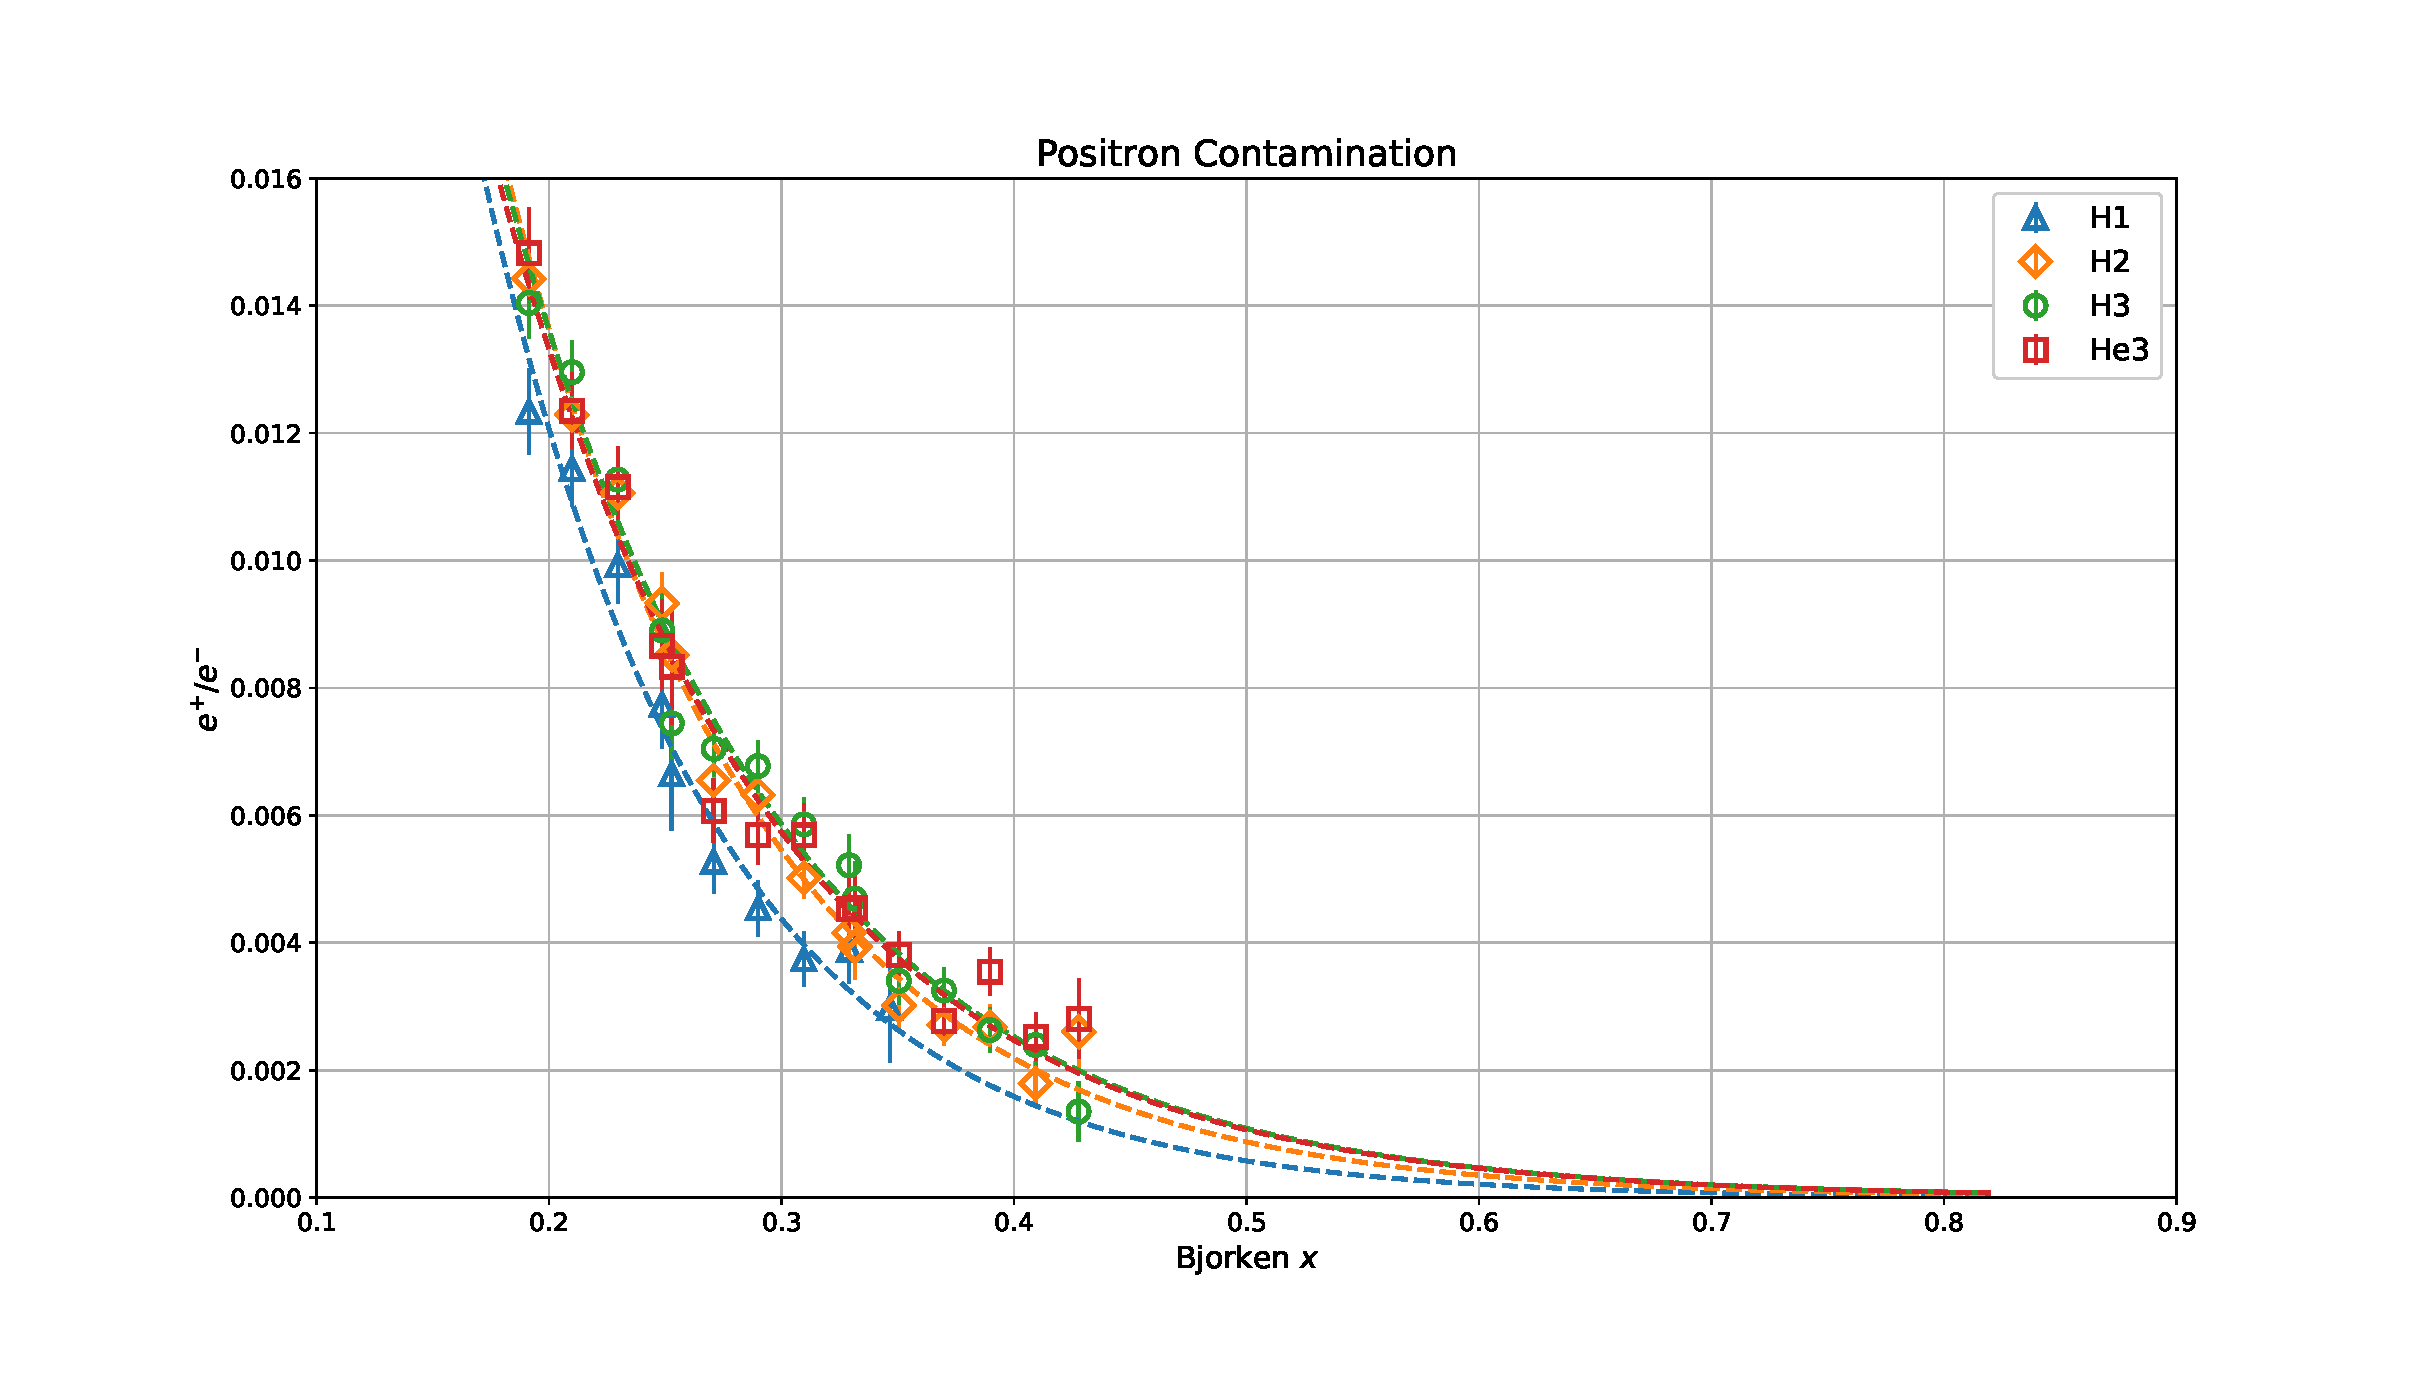
\includegraphics[width=\textwidth]{./analysis/fig/positrons.eps}
	\caption{Charge symmetric background correction}
	\label{fig:positrons}
\end{figure}

\subsection{Computer Deadtime Correction}

Our DAQ unable to continuously record data. While we can probabilistically determine the mean time spacing between events, in the real world events can deviate greatly from these means. Sometimes events will occur that are too close in time for our DAQ to record as the computer has not completed recording the previous event. Deadtime is a function of event rate; when events happen more rapidly, there is a higher chance that events will occur too closely in time to be recorded.

When deadtime is low and the number of recorded events is high, it is a reasonable assumption that the events recorded will accurately reflect the distribution of events in the ``zero-deadtime limit''. In this case correcting for the deadtime is simply done by scaling the number of events by the ``livetime'' of the experiment.

The computer livetime was measured using the Trigger Supervisor and scalers in each HRS. The trigger signals generated from detector signals are copied and sent to both the Trigger Supervisor and a scaler unit. The Trigger Supervisor is subject to the computer deadtime event loss discussed here. The scaler unit, on the other hand, simply increments a register when a trigger signal is received. The ratio of these the number of events recorded by these two systems gives a measure of the livetime of the measurement. The livetime is defined on a run-by-run basis as:

\begin{equation}
DT = \frac{\Sigma \mathrm{Triggers_{TS}}}{\Sigma \mathrm{Triggers_{Scaler}}}
\end{equation}

In an ideal world, the deadtime will be identical for all runs within a kinematic. However, the deadtime is measured on a run-by-run basis and is applied as such in order to account for any deviations from this assumption. The average deadtime for each target in each kinematic is plotted in Figure \ref{fig:deadtime}.

\begin{figure}
	\includegraphics[width=\textwidth]{./analysis/fig/deadtime.eps}
	\caption{Deadtime per kinematic}
	\label{fig:deadtime}
\end{figure}

\subsection{Radiative Corrections}

The Deep Inelastic Cross Sections being studied are the Born approximation of a single-photon exchange. The measurement however, contains contributions from higher order processes that will increase the measured cross section. Using a model, the contributions can be corrected for and removed from the measurement.

The experiment used a software package called $\texttt{T2\_EXTERNALS}$ that calculates both the Born cross section and the radiated cross section for a given target at a kinematic set $(E,E^{\prime} ,\theta )$.

\subsection{Isoscalar Corrections}

\subsection{Bin Centering Corrections}

The cross-section over the width of a bin is not constant. This means that the measurement does not correspond with the true cross section at the center of the bin. Using a model that matches the shape of our data well, the location of the measurement within the bin can be calculated. This is done by calculating the expectation value of the model within that bin and determining the $x$ value corresponding to this value. The expectation value is given by
\begin{equation}
	\langle f_{\rm measured}\rangle = \frac{1}{\Delta x}\int_{x_{\rm low}}^{x_{\rm high}} f\left( x \right) dx,
\end{equation}
where $f$ is a function representing the chosen model. In practice, the $x$ value does not need to be calculated if the data will be reported at the bin center. Rather, the correction is simply the ratio of the model at the bin center. This is written as
\begin{equation}
	\sigma_{\textrm{Bin Centered}} = \frac{f\left(x_{\textrm{Bin Center}}\right)}{\langle f_{\rm measured}\rangle} \sigma_{\rm measured}.
\end{equation}

This correction must be applied to both targets in the ratios. That is, the ratio must be multiplied by the correction to the numerator and divided by the correction to the denominator.\cite{wtsydp}

\subsection{Coulomb Corrections}

Corrections must be made for the effect of the charge of the target on the scattered electron. This interaction causes the $Q^2$ of the event to shift to an effective $Q^2$ value, $Q^2_{\rm eff}$. This conversion is done with the equation
\begin{equation}
	Q^2_{\rm eff} = Q^2 \left(1 + \frac{3Z\alpha\hbar c}{2RE}\right)^{2}.
\end{equation}
In this equation $R$ is the hard-sphere equivalent radius of the nucleus which is defined as $R=\left[\left(\nicefrac{5}{3}\right) \langle r^{2}\rangle\right]^{\nicefrac{1}{2}}$ where $\langle r^2\rangle$ is the root-mean-squared radius of the nucleus.\cite{coulomb}

Using $x=\frac{Q^2}{2M\nu}$, it is clear that a shift in $Q^2$ will result in a proportional shift in $x$. Using a model cross-section, the cross section is calculated at both the nominal $x$ and at $x_{\rm eff}$. As the results have been bin centered, this calculation uses a nominal $x$ at the center of the bin. This will lead to the correction
\begin{equation}
	\sigma_{\textrm{Coulomb Corrected}} = \sigma_{\rm data} \frac{\sigma_{\rm model}\left(x_{\rm eff}\right)}{\sigma_{\rm model}\left(x\right)}.
\end{equation}

This correction must be applied to both targets in the ratios that are calculated.
\subsection{Particle Identification}


%\chapter{\bf{Results}}    % Chapter  4
%%\setcounter{figure}{0}
%%\setcounter{table}{0}
%%\setcounter{equation}{0}
%%\section{Title of First section}
%
%
%\subsection{First subsection}
%
%Here is a Table....
%
%\begin{table}[ht!]
%\caption{Forward Electron Scattering Run Plan}
%\begin{center}
%\begin{tabular}{cccccccc}
%%\multicolumn {7} {c}  {\bf TABLE 4} \\
%\multicolumn {7} {c}  {\bf FORWARD ELECTRON SCATTERING RUN PLAN } \\
%\multicolumn {7} {c}  { } \\ \hline
%$Q^2$  &  $F_C$  & $F_M$ &Cross Section & Time  & Counts & $\Delta F_C$ \\
% (fm$^{-2}$)  &  &  & (cm$^2$/sr) & (hr)  &  & ($\pm\%$) \\ \hline
%    &                     &                     &                           &     &     \\
%12.90 & 3.0$\times 10^{-4}$ & 8.0$\times 10^{-3}$ & 2.7$\times 10^{-34}$ & 1.2 & 12240 & NM  \\
%15.50 & 3.0$\times 10^{-3}$ & 3.4$\times 10^{-3}$ & 5.9$\times 10^{-35}$ & 4.8 & 10800 & 13 \\
%17.50 & 3.5$\times 10^{-3}$ & 1.8$\times 10^{-3}$ & 3.0$\times 10^{-35}$ & 1.2 & 1380  & 9.5 \\
%20.00 & 3.3$\times 10^{-3}$ & 7.0$\times 10^{-4}$ & 1.5$\times 10^{-35}$ & 2.4 & 1360  & 4.1 \\
%22.80 & 2.8$\times 10^{-3}$ & 6.0$\times 10^{-5}$ & 1.4$\times 10^{-35}$ & 1.2 & 630   & 5.4 \\
%26.00 & 2.2$\times 10^{-3}$ & 3.0$\times 10^{-4}$ & 6.4$\times 10^{-36}$ & 4.8 & 1175  & 3.1 \\
%28.00 & 1.8$\times 10^{-3}$ & 4.7$\times 10^{-4}$ & 4.4$\times 10^{-36}$ & 2.4 & 395   & 5.2 \\
%31.50 & 1.3$\times 10^{-3}$ & 5.0$\times 10^{-4}$ & 2.2$\times 10^{-36}$ & 12  & 990   & 11 \\
%35.00 & 9.0$\times 10^{-4}$ & 4.2$\times 10^{-4}$ & 9.9$\times 10^{-37}$ & 9.6 & 360   & 17 \\
%39.25 & 5.5$\times 10^{-4}$ & 3.0$\times 10^{-4}$ & 3.5$\times 10^{-37}$ & 12  & 160   & 25 \\
%43.00 & 3.2$\times 10^{-4}$ & 1.9$\times 10^{-4}$ & 1.1$\times 10^{-37}$ & 19  & 83    & 35 \\
%47.50 & 2.0$\times 10^{-4}$ & 1.1$\times 10^{-4}$ & 3.4$\times 10^{-38}$ & 12  & 16    & NM \\
%Total      &                  &                     &                      & 83  &      &    \\
%           &                  &                     &                      &     &      &  \\ \hline
%\end{tabular}
%\end{center}
%%\caption{Run plan scenario with cross section
%%and counting rate estimates for the forward electron scattering measurements, using the
%%Left HRS system to detect scattered electrons and the BigBite spectrometer to detect
%%recoil triton nuclei in coincidence. (NM means not measurable).}
%\label{table:frp}
%\end{table}
%
%Here is a second Table....
%
%\begin{table}[ht!]
%\caption{Backward Electron Scattering Run Plan}
%%\caption{Backward Electron Scattering Run Plan}
%\begin{center}
%\begin{tabular}{cccccccc}
%%\multicolumn {7} {c}  {\bf TABLE 4} \\
%\multicolumn {7} {c}  {\bf BACKWARD ELECTRON SCATTERING RUN PLAN } \\
%\multicolumn {7} {c}  { } \\ \hline
%$Q^2$  &  $F_C$  & $F_M$ &Cross Section & Time  & Counts & $\Delta F_M$ \\
% (fm$^{-2}$) &  &  & (cm$^2$/sr) & (hr)  &  & ($\pm\%$) \\ \hline
%    &                     &                     &                           &     &     \\
%12.90 & 3.0$\times 10^{-4}$ & 8.0$\times 10^{-3}$ & 9.7$\times 10^{-36}$ & 0.6 & 1080 & 5.2  \\
%15.50 & 3.0$\times 10^{-3}$ & 3.4$\times 10^{-3}$ & 1.7$\times 10^{-36}$ & 2.4 & 885 & 5.6 \\
%17.50 & 3.5$\times 10^{-3}$ & 1.8$\times 10^{-3}$ & 5.8$\times 10^{-37}$ & 0.6 & 86  & 4.6 \\
%20.00 & 3.3$\times 10^{-3}$ & 7.0$\times 10^{-4}$ & 1.7$\times 10^{-37}$ & 4.8 & 226  & 25 \\
%22.80 & 2.8$\times 10^{-3}$ & 6.0$\times 10^{-5}$ & 4.5$\times 10^{-38}$ & 0.6 & 10   & NM \\
%26.00 & 2.2$\times 10^{-3}$ & 3.0$\times 10^{-4}$ & 1.5$\times 10^{-38}$ & 8.5 & 50  & 26 \\
%28.00 & 1.8$\times 10^{-3}$ & 4.7$\times 10^{-4}$ & 1.5$\times 10^{-38}$ & 3.6 & 22   & 15 \\
%31.50 & 1.3$\times 10^{-3}$ & 5.0$\times 10^{-4}$ & 3.7$\times 10^{-38}$ & 4.8  & 48   & 21 \\
%35.00 & 9.0$\times 10^{-4}$ & 4.2$\times 10^{-4}$ & 1.8$\times 10^{-38}$ & 6.0 & 30   & 19 \\
%39.25 & 5.5$\times 10^{-4}$ & 3.0$\times 10^{-4}$ & 6.5$\times 10^{-39}$ & 8.5 & 19   & 18 \\
%43.00 & 3.2$\times 10^{-4}$ & 1.9$\times 10^{-4}$ & 2.1$\times 10^{-39}$ & 15  & 12    & 19 \\
%47.50 & 2.0$\times 10^{-4}$ & 1.1$\times 10^{-4}$ & 5.5$\times 10^{-40}$ & 17  & 4 & 27 \\
%Total      &                  &                     &                      & 72  &      &    \\
%           &                  &                     &                      &     &      &  \\ \hline
%\end{tabular}
%\end{center}
%%\caption{Run plan scenario with cross section
%%and counting rate estimates for the backward electron scattering measurements, using {\it both}
%%HRS systems to detect recoil tritons.
%%The run plan assumes for $Q^2 \ge 2.5$~ (GeV/{\it c})$^2$ a form factor behavior
%% (NM means not measurable).}
%\label{table:brp}
%\end{table}
%
%\subsection{Second subsection}
%
%\subsection{Third subsection}
%


%% If using BibTeX, then comment out the environment below, and
%% provide a \bibliographystyle{} (the 4 standard options are in the
%% preamble above) and a \bibliography{} (the test file template.bib
%% is invoked below).

%\begin{thebibliography}{100}
%%\begin{thebibliography}{99}


\vskip-0.6in
\bibitem{mara} {\it Measurement of the $F_2^n/F_2^p$ and $d/u$ ratios and $A=3$ EMC
effect in deep inelastic scattering off the tritium and helium mirror nuclei},
JLab Proposal PR-12-10-103, J.~Arrington et al., The JLab MARATHON Collaboration, 2010.
\bibitem{CA97} C.~E.~Carlson, J.~R.~Hiller and R.~J.~Holt, Annu. Rev. Nucl.
               Part. Sci. {\bf 47}, 395 (1997).
\bibitem{AL99} L.~C.~Alexa {\it et al.}, Phys. Rev. Lett. {\bf 82},
               1374 (1999); and references therein.
\bibitem{CA13} A.~Camsonne {\it et al.}, {\it Measurement of the $^4$He charge
               form factor at large momentum transfers at Jefferson Lab}, to be
               submitted to Phys. Rev. Lett., May 2013.
\bibitem{KA86} A.~T.~Katramatou, SLAC Report SLAC-NPAS-TN-86-08 (1986).      
\bibitem{PE86} G.~G.~Petratos, SLAC Report NPAS-TN-86-07 (1986).
\bibitem{KA88} A.~T.~Katramatou {\it et al.},
               Nucl. Instrum. Meth. {\bf A267}, 448 (1988).
\bibitem{RITH} K. Rith. 1997. \textit{Lectures on QCD: Applications}. Berlin, Heidelberg: Springer Berlin Heidelberg. \textit{Quark-Gluon Structure of the Nucleon}; p. 250-346.
\bibitem{HaM} F. Halzen, A. Martin. 1984. \textit{Quarks and Leptons: An Introductory Course in Modern Particle Physics}. Wiley.
               
%@Inbook{Rith1997,
%author="Rith, K.",
%editor="Lenz, Frieder
%and Grie{\ss}hammer, Harald
%and Stoll, Dieter",
%title="Quark-gluon structure of the nucleon",
%bookTitle="Lectures on QCD: Applications",
%year="1997",
%publisher="Springer Berlin Heidelberg",
%address="Berlin, Heidelberg",
%pages="250--346",
%isbn="978-3-540-46967-4",
%doi="10.1007/BFb0105861",
%url="http://dx.doi.org/10.1007/BFb0105861"
%}

         
               
%\end{thebibliography}




%\end{thebibliography}
%\bibliographystyle{unsrt}
%\bibliography{bibliography}

%% If using BibTeX (with test file template.bib), uncomment the line below

%\bibliographystyle{plain}
%\bibliographystyle{unsrt}
%\bibliographystyle{alpha}
%\bibliographystyle{abbrv}
%\bibliography{library}

\printbibliography

%% The command below changes numbering from CHAPTER 1, 2, etc. to
%% APPENDIX A, B, etc.

\appendix

%\chapter{\bf{Calibrating the Hall A Raster}}\label{raster_appendix}
%%\setcounter{figure}{0}
%%\setcounter{table}{0}
%%\setcounter{equation}{0}
%\section{What is a Raster Calibration} \label{what}

A well calibrated raster will map a raster current to the instantaneous beam position at both Beam Position Monitors (BPMs) and the target. Accurate beam position data is critical for proper reconstruction of the reaction vertex of physics events. A poorly calibrated horizontal raster will cause poor z-vertex resolution, making it more difficult to subtract the background from target endcaps. A poorly calibrated vertical raster will incorrectly reconstruct event momentum, causing errors in physics analysis.

%The raster calibration can be thought of as defining a line that maps the raster current (measured in ADC bins) to a position.

The raster calibration is completed by defining a function to map the raster current (measured in ADC bins) to a position. The default raster class in the Hall A analyzer uses a linear function for the calibration. Each coil will have two calibration values per position: the slope and intercept of this line. When running in single-arm mode, each raster needs to be calibrated for each arm independently. This is because of differences in performance of the ADCs on each arm. This give a total of twenty-four calibration values as there are three positions (two BPMs and the target) and four coils (two per dimension) calibrated for two arms. When running in coincidence mode, the calibration only needs to be done once since only one arm records the beam data that is used. In this case, there are twelve calibration values. The slope of the line determines the size calibration of the raster coil, the value converts the raster current (in ADC units) to a beam position displaced about the mean beam position. The intercept of the line, in conjunction with the slope, sets this mean beam position. The slope should have units of $meters(m)/$\textit{ADC bin} and the intercept should have units of $meters$.

The Hall A Analyzer software has the capability to include correlation between the x (y) position and the y (x) raster. Historically, this has not been used. There is no evidence that such a correlation exists. This would only come into play if the raster magnets were to shift off-axis (i.e. they rotate so that an electron moving in the z-direction is deflected in a direction that is not purely horizontal or vertical).

The calibration is applied through matrix arithmetic. The raster currents (measured in \textit{ADC Bins}) are represented as a $1\times2$ row matrix. This is then multiplied by the \textit{ADC Bin} to $m$ conversion factor matrix (the slopes of the calibration). This is a $2\times2$ matrix that would only have non-zero off-diagonal elements in the case of an off-axis raster correlation. Finally, the $1\times2$ offset matrix is added to get the final $1\times2$ position matrix.

Equation \ref{cal_apply} shows how the Hall A Analyzer software applies the calibrations. In this equation $R$ represents the raster current, $S$ represents the conversion factor, and $O$ represents the offset. The $l$ indices represent the location of the calibration (i.e. ``A'' for BPMA, ``B'' for BPMB, and ``T'' for target).

\begin{equation}
	\begin{bmatrix}
		^lx & ^ly
	\end{bmatrix}
	=
	\begin{bmatrix}
		^lR_x & ^lR_y
	\end{bmatrix}
	\times
	\begin{bmatrix}
		^lS_{xx} & ^lS_{xy} \\
		^lS_{yx} & ^lS_{yy}
	\end{bmatrix}
	+
	\begin{bmatrix}
		^lO_x & ^lO_y
	\end{bmatrix}
	\label{cal_apply}
\end{equation}

The position at the target is used to determine where the beam is at when intersecting the $z=0$ plane (target center). The positions at the BPMs are used to determine the trajectory of the beam (i.e. at what angle is the beam intersecting the $z=0$ plane). When combined with the interaction plane defined by HRS tracking, the true reaction point can be found. This increases the accuracy of physics reconstruction.

Since only one set of coils is used for physics analysis, that is the only set that is \textit{required} to be calibrated. The method for calibrating the beam position at the target described in this document can only be applied to that particular set of coils. For the Tritium experiments, we used the ``traditional'' method to calibrate the unused set of coils. This was an unnecessary step, as they were never used in analysis; this was done to give us a good starting point in case some unforeseen error required their use.

The second set of coils could be calibrated in this same way by modifying the Rastered Beam class (\textit{THaRasteredBeam}). The data used for physics reconstruction is defined by the THaDetector type class that is added first. By recompiling the analyzer after changing the first raster added, the following calibration methods can be employed for the second set of coils.\cite{Gen}

\section{Determining the Sign of the Calibration}

When determining the beam position, it is obvious to look at the BPM. These are sets of sensing wires in the beamline that can measure the beam position. While the position of the beam reported by the BPMs is highly accurate when averaged over time, the measurement is a slow process and cannot be used on an event-by-event basis. This slowness can cause misleading interpretations of beam movement if we are not careful.

The raster current measures displacement about the central beam position. This measurement says nothing about the \textit{direction} of the displacement. To determine this relation, which is critical to calibrating the rasters, we must use the BPMs and a fixed position feature that we can see in both the BPM and raster spectra: The Carbon Hole target.

To begin, the Carbon Hole must be visible to the beam. Machine Control Center (MCC) is then asked to steer the beam to another BPM position, changing only one dimension. Once there, a short run is taken using the clock trigger. By observing how the carbon hole has moved in the BPM spectrum, the direction that the beam moved can be determined. Note that the MCC BPM coordinate system is not always the same as the hall coordinate system; the BPM data recorded by the Data Acquisition System (DAQ) is in the hall coordinate system. By then observing how the carbon hole moves in the raster spectrum, it can be determined if the coordinate system of the raster in that dimension is the same as that of the BPMs. If the direction of the movement is the same, the sign of the calibration in that dimension is $1$; if the movement is opposite, the sign is $-1$.

This procedure must be completed for both the horizontal and vertical dimensions. The results of this procedure should not change unless the raster power supplies are worked on and wired differently. Under typical circumstances, an experiment only needs to do this procedure once. For the Tritium experiments, we found the sign of the horizontal calibration to be $1$ and the sign of the vertical calibration to be $-1$.\cite{Dien}

\section{Calibrating the Beam Position on Target}

In the past, the calibration values have been found by assuming that the BPMs accurately reflect the mean position and overall magnitude of the rastered beam. By mapping the mean and RMS of raster current to the mean and RMS of BPM positions, a 1:1 mapping could be quickly achieved. Unfortunately, a bandpass filter on the BPM signal prevents the BPMs from accurately reproducing the full size of the rastered beam. We aim to improve on this method to provide the most accurate picture of the beam spread that we can.\cite{bpm_slow}

%Unfortunately, in the Tritium era of Hall A, we have seen that the BPMs no longer accurately reflect the magnitude of the rastered beam. An explanation of this behavior has not been found. Nevertheless, we must find a new calibration method.

While the BPMs can (and still are) used to determine the mean beam position, we must look for other quantities to calibrate the raster size. The obvious choice is the carbon hole target. The carbon hole is used to set the size during data taking because it is known to have a diameter of 2mm. The hole is visible in the raster spectrum, so we can fit it to determine a size calibration for the raster.

The resolution of reconstructed events does not allow for a hard line between the events originating from the foil and the absence of events in the ``hole'' region. Events smear across this border suggesting that we ought to use a smooth function to define the edge. We decided to use a radial sigmoid function with a floating ``hardness'' constant. A sigmoid, shown in equation \ref{eqn:base_sig}, is a smoothed step function with a constant that determines how hard of a step it is. In this general form of the equation, $a$ is the vertical axis and $b$ is the horizontal axis. As shown in Figure \ref{fig:sighard}, a sigmoid approaches a step function as the ``hardness'' constant approaches infinity. This was found to converge\footnote{When doing these fits, be sure to the Log Likelihood method} and visually appears to fit the hole well. This fitting procedure determines the edge of the hole to be at the position where the value is halfway between the minimum and maximum value of function.\cite{Evan}

\begin{figure}
	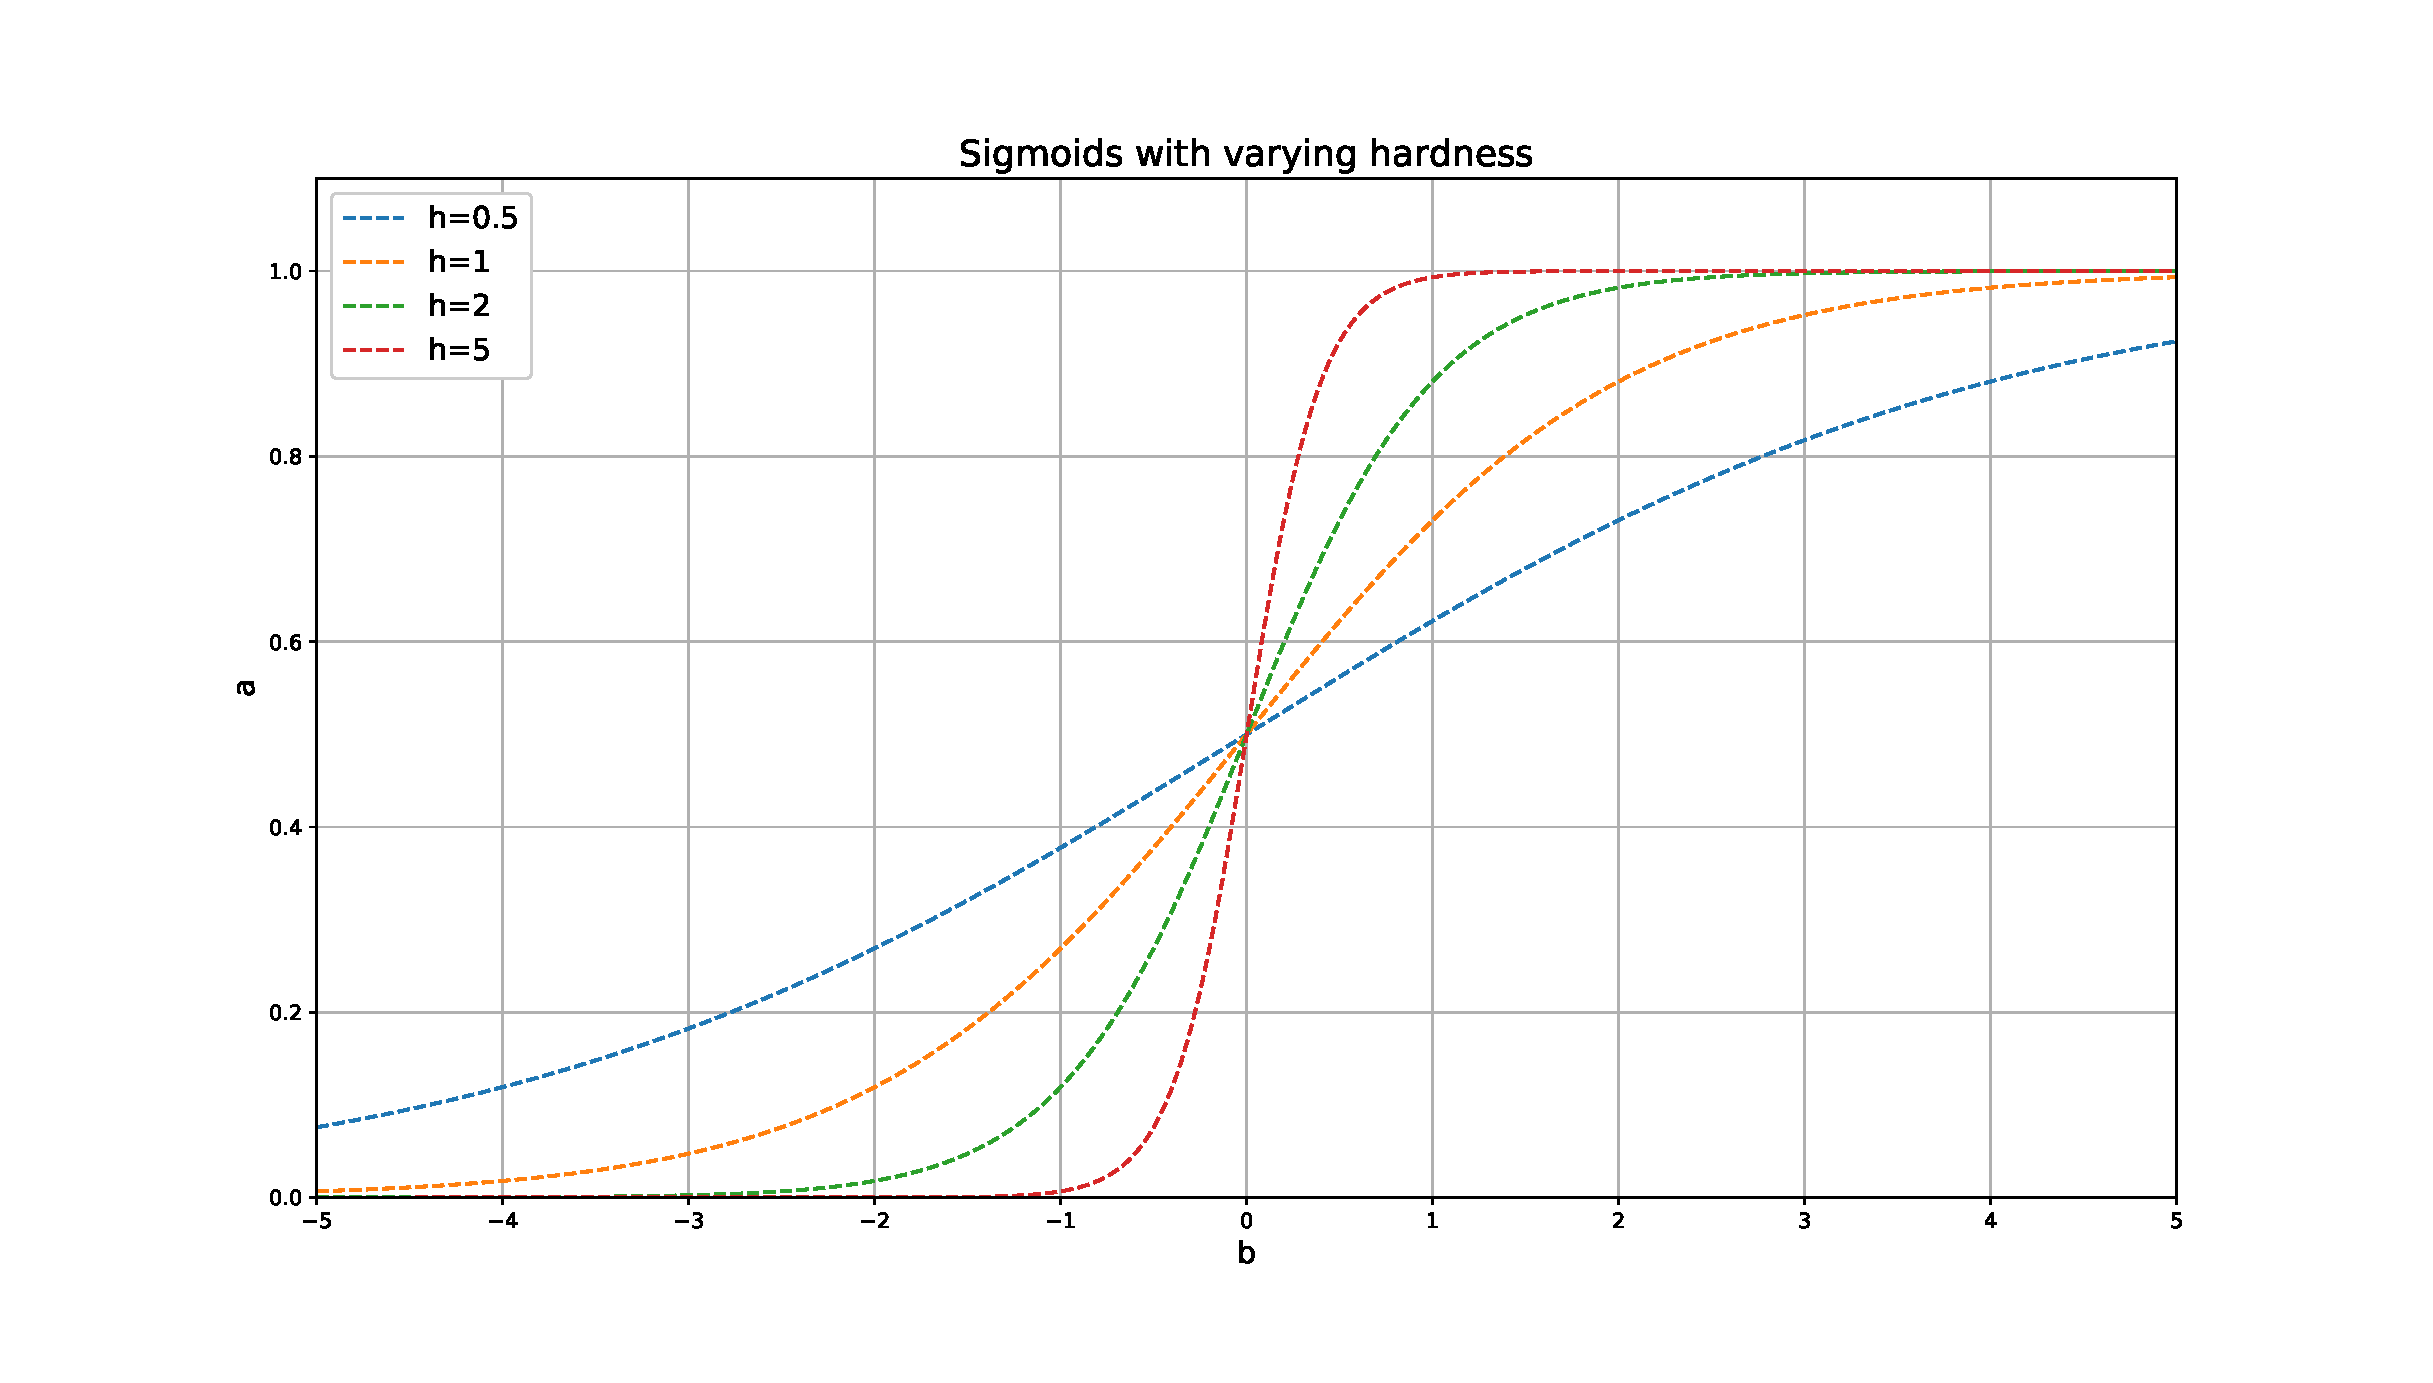
\includegraphics[width=\textwidth]{./app1/figures/sig_hard.eps}
	\caption{A 1 Dimensional Sigmoid Function with Varying Hardness Parameter}
	\label{fig:sighard}
\end{figure}

\begin{equation}
	a = \frac{1}{1 + e^{-h\cdot b}}
	\label{eqn:base_sig}
\end{equation}


Equation \ref{eqn:radsig} describes the sigmoid that we use to fit the carbon hole. In the equation, ``Counts'' is the counts in a given bin, $x$ is the horizontal raster value (in ADC bins), and $y$ is the vertical raster value (in ADC bins). For definitions of the fit parameters $p0$ through $p6$, see table \ref{tbl:sigvar_desc}. For this fit, the conversion factors are restricted to positive numbers in a small region around an ``educated guess'' of the approximate conversion factors. These ``educated guesses'' can be determined by roughly measuring, by eye, the approximate width of the carbon hole in \textit{ADC bins} and then dividing by $2mm$. The center values are restricted to the approximate range of the raster data. These restrictions ensure that the fit is not fooled by any outlying data, which can be readily determined by eye when the fit is drawn. The sign of the calibration needs to be applied (multiplicatively) to ensure the calibration is done correctly.

\begin{equation}
\mathrm{Counts} = \frac{p0}{1+e^{-p5*\left(\left(p1*\left(p2-x\right)\right)^{2}+\left(p3*\left(p4-y\right)\right)^{2}-1\right)}}+p6
\label{eqn:radsig}
\end{equation}

\begin{center}
\begin{tabulary}{0.9\textwidth}{|L|L|}
	\multicolumn{2}{c}{\textbf{Parameter Definitions}}
	\\
	\hline
	$p0$ & Approximate signal level outside the carbon hole (measured in ADC bins)\\
	$p1$ & Current (ADC bins) to $mm$ conversion factor for Horizontal Raster\\
	$p2$ & Horizontal center of the carbon hole in current (ADC) units\\
	$p3$ & Current (ADC bins) to $mm$ conversion factor for Vertical Raster\\
	$p4$ & Vertical center of the carbon hole in current (ADC) units\\
	$p5$ & ``Hardness'' factor for the sigmoid (approaches a step function as this increases)\\
	$p6$ & Approximate signal level inside the carbon hole (measured in ADC bins)\\
	\hline
\end{tabulary}
\label{tbl:sigvar_desc}
\end{center}

Note that in equation \ref{eqn:radsig}, the fit conversion factor will have units of $mm/$\textit{ADC bin}. The resulting conversion factors must be divided by 1000 before further use. This was done for clarity as the size of the Carbon Hole is typically discussed in $mm$. To avoid the need for further unit conversion, the following equation can be used instead.

\begin{equation}
\mathrm{Counts} = \frac{p0}{1+e^{-p5*\left(\left(p1*\left(p2-x\right)\right)^{2}+\left(p3*\left(p4-y\right)\right)^{2}-10^{-6}\right)}}+p6
\label{eqn:radsig_m}
\end{equation}

\begin{figure}
	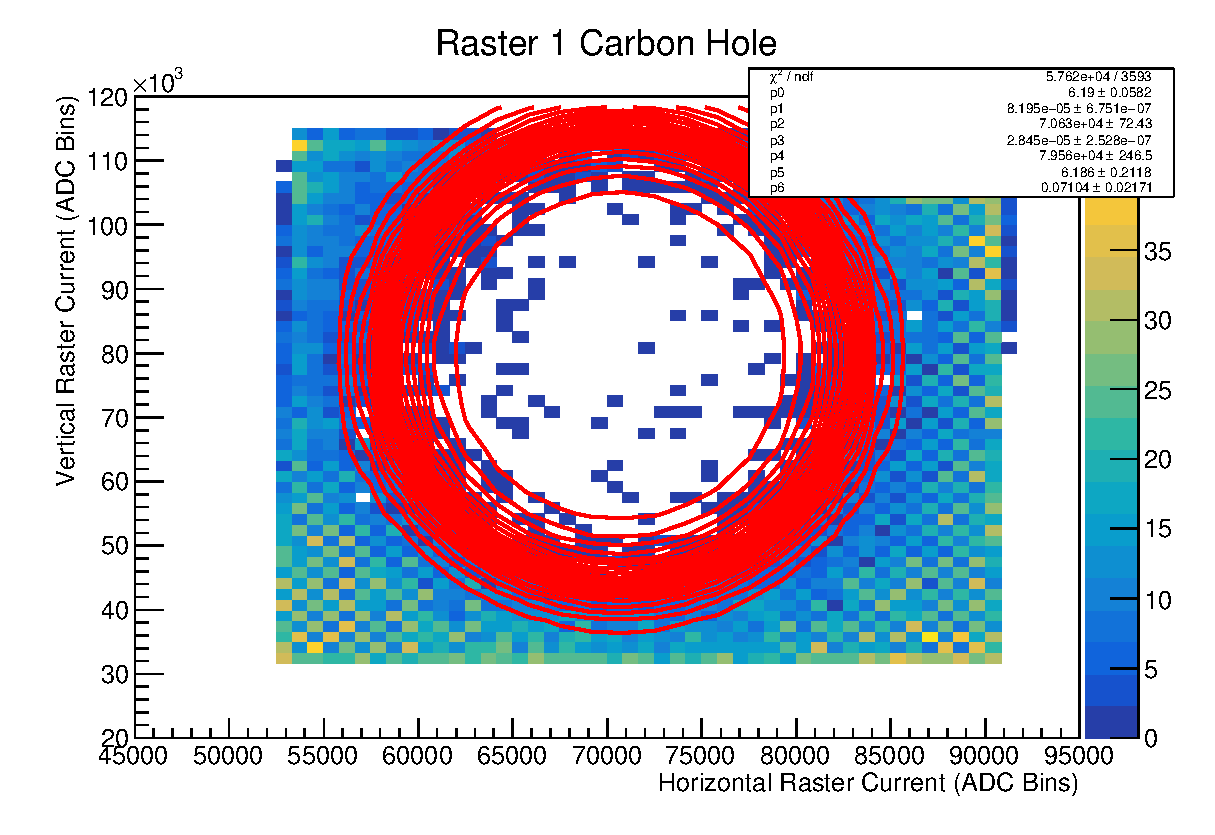
\includegraphics[width=\textwidth]{./app1/figures/hole_fit.eps}
	\caption{Using the radial sigmoid function to fit the hole in the Carbon Hole target. In this plot, the density of red rings is directly correlated to the slope of the function at that point. Where the rings are densest is the 50\% position, corresponding to where the fit locates the edge of the hole.}
	\label{fig:carbholefit}
\end{figure}

Upon further analysis, it was determined that this calibration method yielded little improvement over the ``traditional'' method. The fit places the edge of the hole at the horizontal zero-crossing of the sigmoid function. Due to smearing from the spectrometer, this is not the ``true edge'' of the hole. This was determined by looking at the physics values that the raster calibration affects. For the horizontal rasters, this is the reconstructed z position at the target. For the vertical rasters, this is W$^2$. When the rasters are properly calibrated, there should be no correlations between the raster current and the physics variables that are affected by the calibration.

Proceeding further, we determined that we ought to look at these physics values for improving the calibration. Utilizing two ``bad'' calibrations, we looked at the strength of the correlation as it is related to the calibration. If we assume that the relation is linear, we can interpolate (or extrapolate if they were bad in the same direction) to determine the correct calibration.\cite{Rey}

For the horizontal raster, we used the single carbon foil target and plot the horizontal raster current versus the reconstructed z position. We can then take slices of this plot in horizontal raster current bins and fit the resulting plots with a Gaussian and plot the peaks. With a properly calibrated raster, there should be no correlation between horizontal raster current and reconstructed z. Using two improper horizontal calibrations, we measured the slopes of the correlations. We then interpolated to determine the calibration that would yield a slope of 0. This procedure forces the sign of the calibration to be built into the answer, there is no need to apply it.

In practice, this does not yield a calibration with a slope of \textit{precisely} zero. This is due to statistical fluctuations in the data around the true correlation line. We attempted to iterate this procedure, but it did not yield significant improvement on the results.

\begin{figure}
	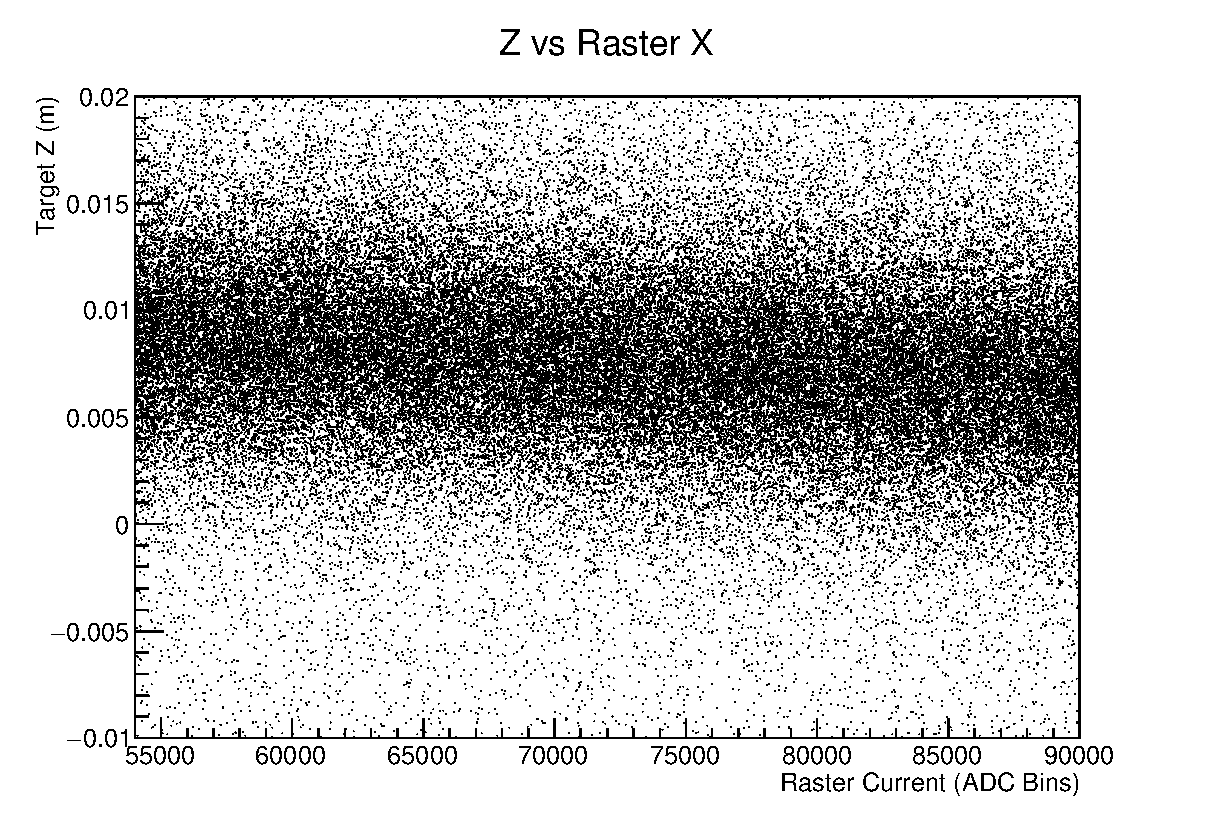
\includegraphics[width=\textwidth]{./app1/figures/old1_zvx.eps}
	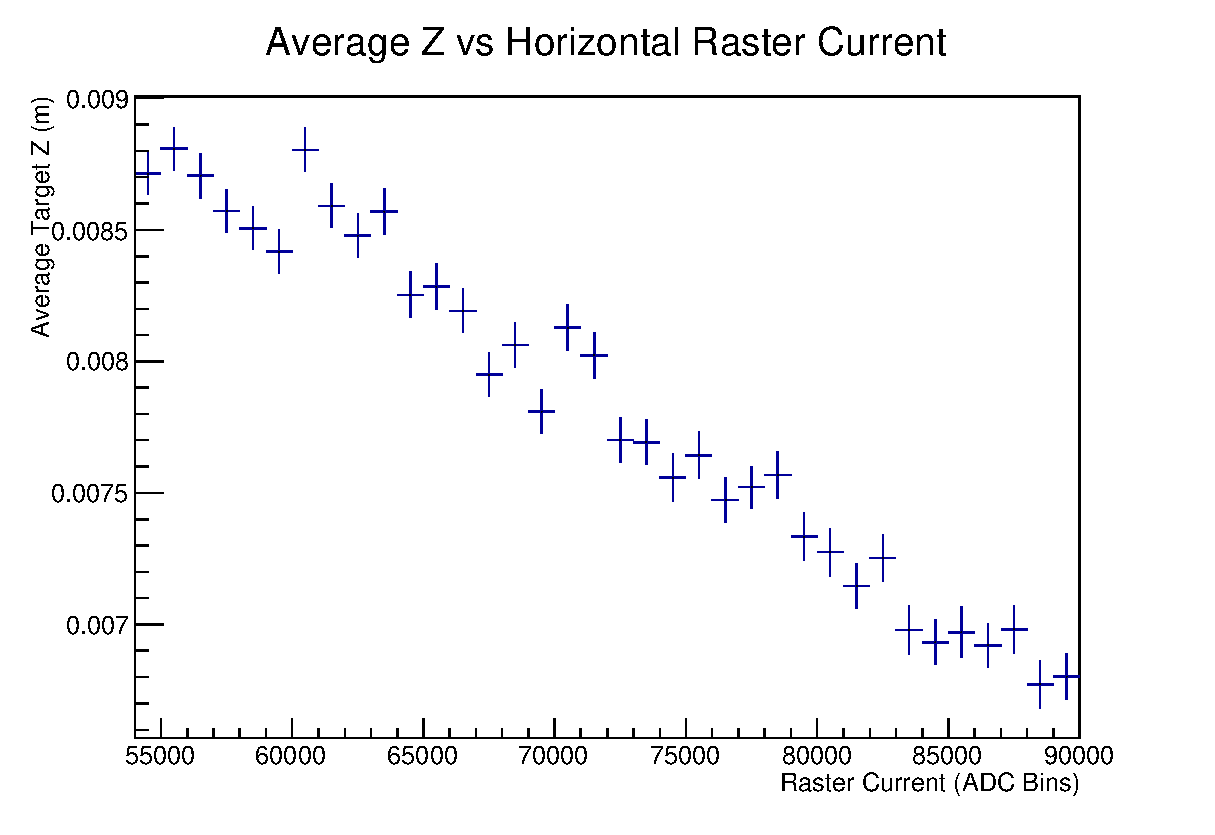
\includegraphics[width=\textwidth]{./app1/figures/old1_avgzvx_nofit.eps}
	\caption{Slices in horizontal raster current of the reconstructed z versus raster current plot are fit with a Gaussian. The peaks of the Gaussian are then plotted to see the correlation. In the plot of average z, it can be seen that the peak position shifts by over 2mm over the movement of the raster. The carbon foil is only 0.25mm thick.}
\end{figure}

\begin{figure}
	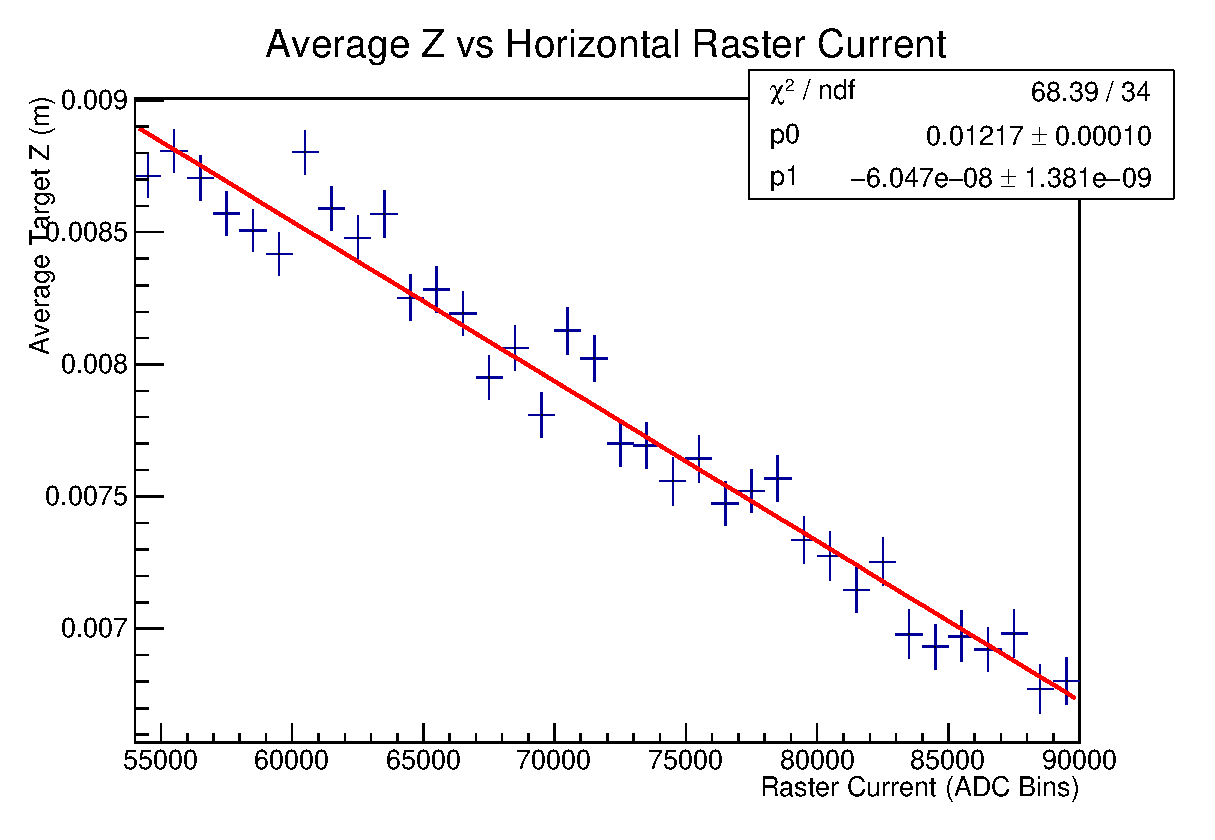
\includegraphics[width=\textwidth]{./app1/figures/old1_avgzvx.eps}
	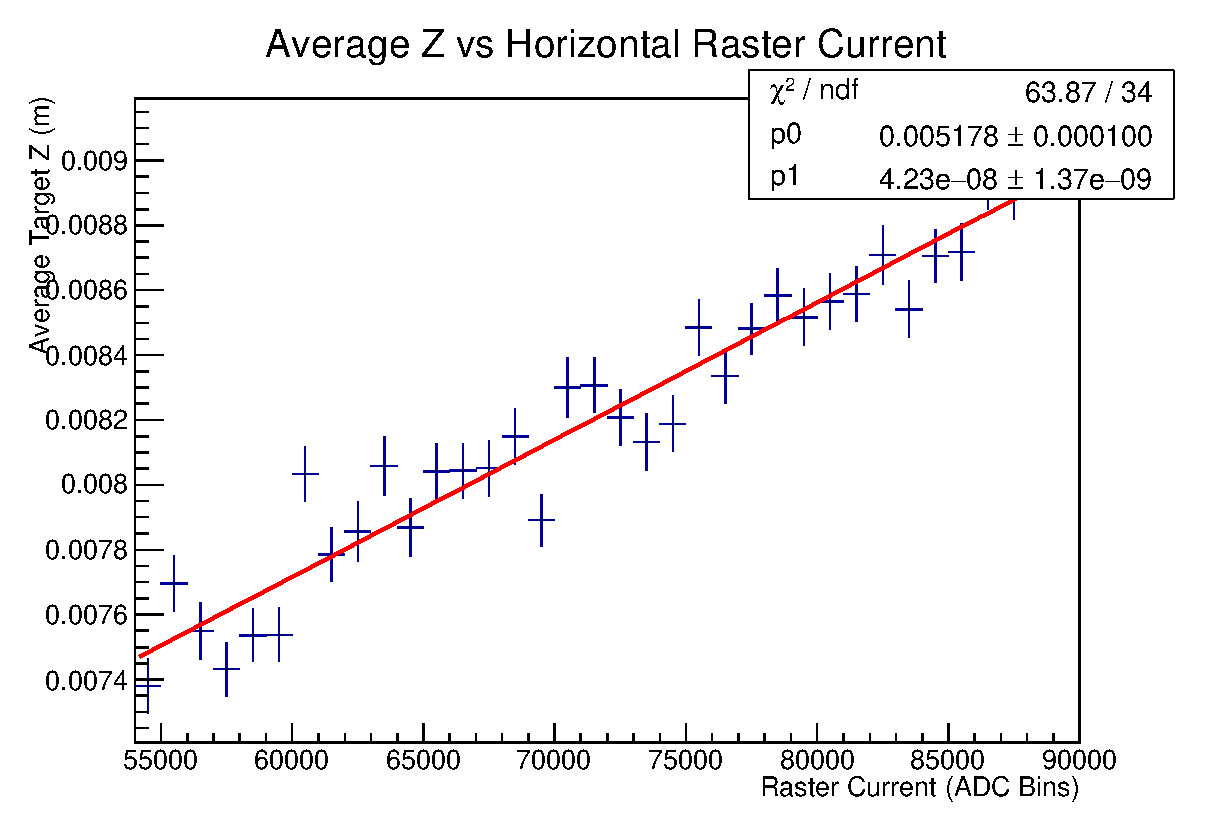
\includegraphics[width=\textwidth]{./app1/figures/old2_avgzvx.eps}
	\caption{Two ``bad'' calibrations are fit to find the correlation between horizontal raster current and the average x position. Both of these calibrations show a displacement larger than the thickness of the target.}
\end{figure}
\begin{figure}
	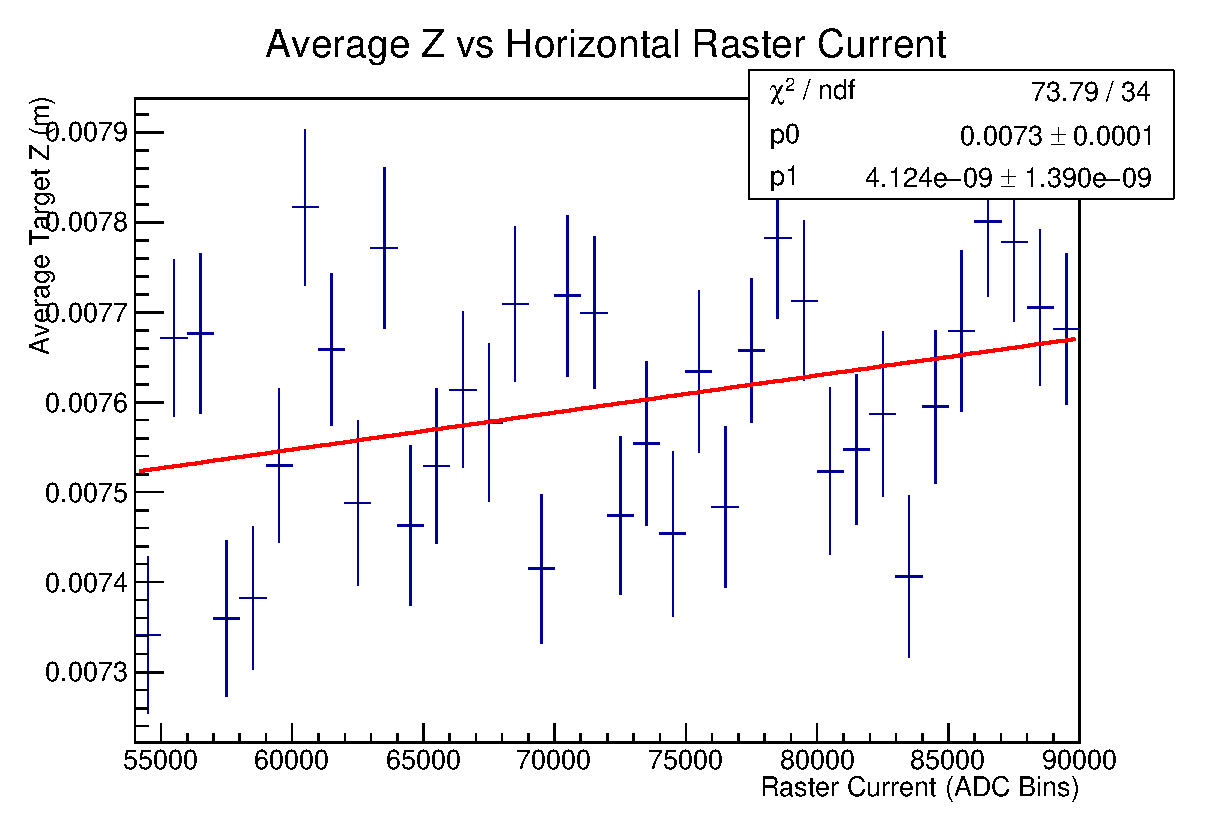
\includegraphics[width=\textwidth]{./app1/figures/avgzvx.eps}
	\caption{Using a linear fit of the correlation between average z and horizontal raster current for two ``bad'' calibrations, we can interpolate to the correct calibration. Here we can see that the shift is approximately 0.1mm.}
\end{figure}

For the vertical raster, we look for a momentum feature that the experiment can see. In the case of many of the Tritium era experiments, the Hydrogen elastic peak was measured. Plotting the vertical raster current versus the W$^2$ of Hydrogen elastic events, we followed a similar procedure to that of the horizontal raster. As with the horizontal calibration, there is no need to apply the sign of the calibration in this method.

For experiments that do not have an identifiable momentum feature, an approximation of the correct vertical calibration can be found using the horizontal calibration and the sigmoid fit of the carbon hole. Since it is known that the true calibration lies somewhere on the sigmoid above the zero-crossing, we can use the horizontal calibration to determine where that point is. To do this, we determine how many horizontal ADC bins away from center the ``true edge'' lies using the calibration determined using the z vertex reconstruction (the ``true edge'' is $1mm$ away from the center). We then evaluate equation \ref{eqn:radsig} using this value. Then, equation \ref{eqn:radsig} is reversed to determine the vertical ADC bin displacement to yield the same value. Once we have the displacement, a new vertical calibration can be determined. This is an imperfect solution, but ultimately should provide the best calibration possible in the absence of a momentum feature.

Once these methods are used to determine the slope of the raster calibration, we turn our attention back to the BPMs. The BPMs, after calibration with the harp, provide a very accurate reading of the mean beam position at their location in the beamline. This information can then be used to determine the mean position of the beam at the target. To do this, we plot each BPMs position spectrums and determine the mean value. Each spectrum must have its mean determined independently because the BPM readings lag behind events, the position is only accurate when averaged over time. Once we know the mean positions at each BPM, a track through the means can be projected to the mean position at the target.

With the slope of the raster calibrations and a point on the calibration lines (the mean position at the target), we have all the information that we need to determine the raster calibration lines. Using a simple point-slope form, we input the information for each raster and solve for the intercept.

\section{Calibrating the Beam Position at the BPMs}

The beam position must also be calibrated at the BPMs. To do this, we use the ``traditional'' method of raster calibration. As in determining the mean position at the target, the raster and BPM spectrums are plotted. The means and RMS of each spectrum are then calculated. In these cases, since we are determining the calibration at the BPMs, no projection is needed.

To determine the size calibration, the slope of the calibration line, divide the RMS of the BPM spectrum by the RMS of the raster spectrum and then multiply by the sign of the calibration. To then determine the calibration offset, point-slope form of a line can be implemented using the mean positions and the aforementioned slope calculation.\cite{Barak}

\end{document}
